\documentclass[a4paper]{scrbook}

\usepackage[utf8]{inputenc}
\usepackage{graphicx}
\usepackage{booktabs}
\usepackage{url}
\usepackage{relsize}
\usepackage{hyperref}
\usepackage{libertine}
\usepackage{ifthen}
\usepackage{float}
\usepackage{enumerate}
\usepackage{enumitem}
\usepackage{tabularx}
\usepackage{adjustbox}
\usepackage{amsmath,amssymb,amsfonts}
\usepackage{setspace}
\usepackage{caption}
\usepackage{subcaption}
\usepackage{xcolor}
\usepackage{cite} 
\usepackage{algorithm}
\usepackage{algpseudocode}
\usepackage{array}
\usepackage{textcomp}
\usepackage{anyfontsize}
\usepackage{pifont}
\usepackage{amssymb} 
\usepackage{pgfplots}
\usepackage{listings}


\pgfplotsset{compat=1.18}


\lstset{
    language=Python,
    basicstyle=\ttfamily\small,
    keywordstyle=\color{blue},
    stringstyle=\color{orange},
    commentstyle=\color{gray},
    frame=single,
    breaklines=true,
    columns=flexible,
    backgroundcolor=\color{gray!5},
    captionpos=b
}



\onehalfspacing  
\KOMAoptions{open=any}


% \usepackage{cite} 

\raggedbottom

% \usepackage{fancyhdr}
% \KOMAoptions{open=any}


%%%%%%%%%%%%%%%%%%%%%%%%%%%%%%%%%%%%%%%%%%%%%%%%%%%%%%%%%%%%%%%%%%%%%%%%%%%%%%%%
% Replace these values
%%%%%%%%%%%%%%%%%%%%%%%%%%%%%%%%%%%%%%%%%%%%%%%%%%%%%%%%%%%%%%%%%%%%%%%%%%%%%%%%
\newcommand{\thesistitleDE}{Erzeugung optischer Fernerkundungsdaten (Sentinel-2) auf Basis von Radar-Fernerkundungsdaten (Sentinel-1) mittels generativer KI}
\newcommand{\thesistitleEN}{Generation of optical remote sensing data (Sentinel-2) based on radar remote sensing data (Sentinel-1) using generative AI}

\newcommand{\student}{Ahmed Attia}
\newcommand{\matrnr}{00815907}
\newcommand{\stammnr}{} % Unset this variable if you only have a (single) matriculation number
% \newcommand{\stammnr}{234567} % Unset this variable if you only have a (single) matriculation number
\newcommand{\submissiondate}{XX.\ Monat 20XX}
\newcommand{\supervisor}{Dr. Peter Hofmann}
\newcommand{\secsupervisor}{} % Unset this variable if no second supervisor is required
% \newcommand{\secsupervisor}{Prof.~Dr.~Zweitprüfer} % Unset this variable if no second supervisor is required
\newcommand{\faculty}{Angewandte Informatik}

% Select your course of studies here
\newcommand{\studies}{Bachelor Künstliche Intelligenz}
\newcommand{\degree}{Bachelor of Science (B.Sc.)}
%%%%%%%%%%%%%%%%%%%%%%%%%%%%%%%%%%%%%%%%%%%%%%%%%%%%%%%%%%%%%%%%%%%%%%%%%%%%%%%%

\renewcommand*{\UrlFont}{\ttfamily\smaller\relax}

\begin{document}
\pagestyle{headings}
\pagenumbering{roman}


% % Erklärung über die Selbständigkeit der Arbeit
\thispagestyle{empty}
\newcommand{\signature}[1]{%
\bigskip
\noindent
\begin{tabular*}{\linewidth}{lp{3cm}p{1cm} p{6cm}}
Deggendorf, & \dotfill & & \dotfill \\
& {\footnotesize Datum} & & {\centering \footnotesize #1}
\end{tabular*}
}

\begin{minipage}[b]{.5\linewidth}
	\Large\textbf{Erklärung}
\end{minipage}
\begin{minipage}[b]{.5\linewidth}
	
\includegraphics[width=\linewidth]{img/THD_Logo.pdf}
\end{minipage}

\bigskip

Name des Studierenden: \quad \student

\bigskip
Name des Betreuenden: \quad \supervisor

\vspace{.7cm}
Thema der Abschlussarbeit:

\vspace{.5em}
{\def\\{\relax\ifhmode\unskip\fi\space\ignorespaces}
\thesistitleDE
}\dotfill

\vspace{.5em}
\dotfill

\vspace{.5em}
\dotfill

\vspace{.5em}
\dotfill

\begin{enumerate}
	\item Ich erkläre hiermit, dass ich die Abschlussarbeit gemäß § 35 Abs.~7 RaPO (Rahmen\-prüf\-ungs\-ordnung für die Fachhochschulen in Bayern, BayRS 2210-4-1-4-1-WFK)  selbständig  verfasst,  noch  nicht  anderweitig  für Prüfungszwecke  vorgelegt,  keine  anderen  als  die  angegebenen  Quellen  oder Hilfsmittel  benutzt  sowie  wörtliche  und  sinngemäße  Zitate  als  solche gekenn\-zeichnet habe.

		\signature{Unterschrift des Studierenden}

	\item  Ich  bin  damit  einverstanden, dass die von  mir angefertigte  Abschlussarbeit über die Bibliothek der Hochschule einer breiteren Öffentlichkeit zugänglich gemacht wird:
		\begin{itemize}
			\item[$\bigcirc$] Nein
			\item[$\bigcirc$] Ja, nach Abschluss des Prüfungsverfahrens
			\item[$\bigcirc$] Ja, nach Ablauf einer Sperrfrist von \ldots Jahren.
		\end{itemize}

		\signature{Unterschrift des Studierenden}
\end{enumerate}

\noindent
\hrulefill

{\centering{\footnotesize Bei Einverständnis des Verfassenden vom Betreuenden auszufüllen:}}

{\flushleft

Eine Aufnahme eines Exemplars der Abschlussarbeit in den Bestand der Bibliothek und die Ausleihe des Exemplars wird:

\begin{itemize}
	\item[$\bigcirc$] Befürwortet
	\item[$\bigcirc$] Nicht befürwortet
\end{itemize}

		\signature{Unterschrift des Betreuenden}
}

% \cleardoublepage\par
\clearpage

\setkomafont{title}{\Large \scshape}
\begin{titlepage}
\begin{center}
	{\usekomafont{subject}
	Technische Hochschule Deggendorf\\
	Fakultät \faculty\par}
	\vspace{.2cm}
{\Large \studies\\}
% {\Large Studiengang \studies\\}
\vspace{6\baselineskip}
{\usekomafont{title}\thesistitleDE\par}
\vspace{1cm}
{\usekomafont{title}\thesistitleEN\par}
\vspace{6\baselineskip}

\usekomafont{publishers}
Bachelorarbeit zur Erlangung des akademischen Grades:
% Masterarbeit zur Erlangung des akademischen Grades:

	\vspace{.2cm}
	\emph{\degree}
	\vspace{.2cm}

an der Technischen Hochschule Deggendorf\\
\end{center}
\vfill
\parbox[t]{.4\textwidth}{\usekomafont{author}
	Vorgelegt von:\\
	\student\\
	Matrikelnummer: \matrnr\par
	\ifthenelse{\equal{\stammnr}{}}{}{
	Stammnummer: \stammnr\par
	}
	\vspace{\baselineskip}
	Am: \submissiondate\par
}
\hfill
\parbox[t]{.4\textwidth}{\usekomafont{author}
Prüfungsleitung:\\
\supervisor%

\ifthenelse{\equal{\secsupervisor}{}}{}
{%
\vspace{\baselineskip}
Ergänzende Prüfende:\\
\secsupervisor%
}}
\end{titlepage}
\cleardoublepage\par
% \clearpage\par
\begingroup
\setstretch{1.0}
% Erklärung über die Selbständigkeit der Arbeit
\thispagestyle{empty}
\newcommand{\signature}[1]{%
\bigskip
\noindent
\begin{tabular*}{\linewidth}{lp{3cm}p{1cm} p{6cm}}
Deggendorf, & \dotfill & & \dotfill \\
& {\footnotesize Datum} & & {\centering \footnotesize #1}
\end{tabular*}
}

\begin{minipage}[b]{.5\linewidth}
	\Large\textbf{Erklärung}
\end{minipage}
\begin{minipage}[b]{.5\linewidth}
	
\includegraphics[width=\linewidth]{img/THD_Logo.pdf}
\end{minipage}

\bigskip

Name des Studierenden: \quad \student

\bigskip
Name des Betreuenden: \quad \supervisor

\vspace{.7cm}
Thema der Abschlussarbeit:

\vspace{.5em}
{\def\\{\relax\ifhmode\unskip\fi\space\ignorespaces}
\thesistitleDE
}\dotfill

\vspace{.5em}
\dotfill

\vspace{.5em}
\dotfill

\vspace{.5em}
\dotfill

\begin{enumerate}
	\item Ich erkläre hiermit, dass ich die Abschlussarbeit gemäß § 35 Abs.~7 RaPO (Rahmen\-prüf\-ungs\-ordnung für die Fachhochschulen in Bayern, BayRS 2210-4-1-4-1-WFK)  selbständig  verfasst,  noch  nicht  anderweitig  für Prüfungszwecke  vorgelegt,  keine  anderen  als  die  angegebenen  Quellen  oder Hilfsmittel  benutzt  sowie  wörtliche  und  sinngemäße  Zitate  als  solche gekenn\-zeichnet habe.

		\signature{Unterschrift des Studierenden}

	\item  Ich  bin  damit  einverstanden, dass die von  mir angefertigte  Abschlussarbeit über die Bibliothek der Hochschule einer breiteren Öffentlichkeit zugänglich gemacht wird:
		\begin{itemize}
			\item[$\bigcirc$] Nein
			\item[$\bigcirc$] Ja, nach Abschluss des Prüfungsverfahrens
			\item[$\bigcirc$] Ja, nach Ablauf einer Sperrfrist von \ldots Jahren.
		\end{itemize}

		\signature{Unterschrift des Studierenden}
\end{enumerate}

\noindent
\hrulefill

{\centering{\footnotesize Bei Einverständnis des Verfassenden vom Betreuenden auszufüllen:}}

{\flushleft

Eine Aufnahme eines Exemplars der Abschlussarbeit in den Bestand der Bibliothek und die Ausleihe des Exemplars wird:

\begin{itemize}
	\item[$\bigcirc$] Befürwortet
	\item[$\bigcirc$] Nicht befürwortet
\end{itemize}

		\signature{Unterschrift des Betreuenden}
}

% \cleardoublepage\par
\clearpage

\endgroup


\tableofcontents
\listoffigures
\listoftables

\chapter*{List of Abbreviations}
% \addcontentsline{toc}{chapter}{List of Abbreviations}

\begin{table}[h!]
\centering
\begin{tabular}{ll}
\textbf{Abbreviation} & \textbf{Full Form} \\
\midrule
RS      & Remote Sensing \\
SAR     & Synthetic Aperture Radar \\
GAN     & Generative Adversarial Network \\
cGAN    & Conditional Generative Adversarial Network \\
CNN     & Convolutional Neural Network \\
DDPM    & Denoising Diffusion Probabilistic Model \\
ESA     & European Space Agency \\
GRD     & Ground Range Detected \\
EW      & Extra-Wide Swath Mode \\
IW      & Interferometric Wide Swath Mode \\
WV      & Wave Mode \\
LULC    & Land Use and Land Cover \\
MODIS   & Moderate Resolution Imaging Spectroradiometer \\
ROI     & Region of Interest \\
SWIR    & Shortwave Infrared \\
VNIR    & Visible and Near Infrared \\
VV      & Vertical–Vertical Polarization \\
VH      & Vertical–Horizontal Polarization \\
NIR     & Near Infrared \\
IQA     & Image Quality Assessment \\
SSIM    & Structural Similarity Index Measurement \\
FSIM    & Feature Similarity Index Measurement \\
FSIM    & Image Quality Assessment \\
DISTS   & Deep Image Structure and Texture Similarity \\
PSNR    & Peak Signal-to-Noise Ratio \\
SAM     & Spectral Angle Mapper \\
FID     & Fréchet Inception Distance \\
LPIPS   & Learned Perceptual Image Patch Similarity \\
BCE     & Binary Cross-Entropy \\
\end{tabular}
\end{table}

% \chapter*{Abstract}
\addcontentsline{toc}{chapter}{Abstract}
% \cleardoublepage

\setcounter{page}{1}
\pagenumbering{arabic}


% \chapter{Introduction}

Earth observation has become an indispensable tool for understanding and monitoring the planet’s dynamic processes. Optical and radar remote sensing represent two complementary modalities at the core of modern Earth observation systems. Optical sensors provide rich spectral and visual information suitable for human interpretation. This information is used, among others, in forest prediction, agricultural monitoring, military, etc~\cite{S2MS_GAN}. However, they are inherently constrained by atmospheric conditions such illumination variability and in particular cloud cover. This causes considerable data gaps in both the spatial and temporal domains~\cite{CR_SEN2_dRNN}. 
In contrast, synthetic aperture radar (SAR) sensors operate in the microwave domain, offering all-weather, day-and-night imaging capabilities independent of sunlight or cloud interference. However, the backscatter-based nature of SAR imagery introduces challenges related to speckle noise, geometric distortions, and the absence of spectral color information~\cite{bench_sar_color, naderi2021}, complicating its interpretation.

To bridge the gap between these two sensing modalities, SAR-to-optical image translation has emerged as a powerful generative approach. It aims to synthesize optical-like, cloud-free imagery from SAR data, combining the interpretability of optical observations with the robustness of radar acquisitions. Recent advances in generative artificial intelligence (GenAI), particularly in conditional generative adversarial networks (cGANs) and diffusion models, have made it possible to learn complex mappings between SAR and optical domains with remarkable realism~\cite{cr_fuse_HR_GEN}. 
These developments have opened new pathways for applications in land-cover classification, vegetation monitoring, disaster response, and particularly, cloud removal. % keep or delete?

Despite the rapid progress in this field, most existing studies have focused primarily on reconstructing the visible RGB subset of optical imagery, with a few extending to the NIR range, leaving the full multispectral potential of missions such as Sentinel-2 largely underexplored. Furthermore, while SAR-to-optical translation is often evaluated qualitatively, systematic assessments of its reliability across individual spectral bands remain limited. Finally, although the approach shows promise for cloud removal, its effectiveness in this context has not yet been comprehensively validated across the full spectral range

Against this background, the present thesis investigates the use of generative models for translating Sentinel-1 SAR imagery into multispectral Sentinel-2 optical data. The work is guided by three main objectives:
\begin{enumerate}
    \item To validate SAR-to-optical image translation across the full 13 Sentinel-2 spectral bands. 
    \item To assess how reliably each optical band can be individually reconstructed and to what extent.
    \item To evaluate the performance of SAR-to-optical image translation for cloud removal
\end{enumerate}

Through these objectives, this thesis aims to provide a comprehensive and quantitative understanding of SAR-to-optical translation as a multimodal learning problem, highlighting its strengths, limitations, and potential for operational cloud-free optical data generation.

\bigskip
\textcolor{red}{layout the thesis}
% \noindent
% \textbf{Thesis Structure.}
The remainder of this thesis is organized into six chapters, each addressing a distinct component of the research.
Chapter~\ref{ch:background} provides the theoretical background and literature review, introducing the fundamentals of remote sensing, the Copernicus Sentinel missions, cloud removal methodologies, and generative artificial intelligence for multimodal data fusion.
Chapter~\ref{ch:methodology} outlines the methodological framework, including the problem formulation, dataset selection, preprocessing pipeline, and the design of the \textit{Pix2Pix} model together with its training and evaluation procedures.
Chapter~\ref{ch:results} presents the experimental results and analyses, covering the main evaluation scenarios: reconstruction on partial and full datasets, per-band performance assessment, and validation on cloud removal tasks.
Chapter~\ref{ch:ablation} reports the ablation studies that examine the effect of different loss functions and the exclusion of specific spectral bands, providing a deeper understanding of the model’s behavior.
Chapter~\ref{ch:challenges} discusses the main challenges encountered during experimentation, such as training instability and artifact formation, along with the corrective strategies implemented.
Finally, Chapter~\ref{ch:limitations} concludes the work by summarizing its limitations and outlining future research directions, including temporally generalized learning, diffusion-based architectures, and band-aware normalization strategies.
Supplementary material, such as per-band reconstructions and seasonal evaluations, is included in the appendices.

The remainder of this thesis is organized as follows.
Chapter~\ref{ch:background} introduces the theoretical background, including remote sensing fundamentals, the Sentinel missions, cloud removal methods, and generative AI approaches.
Chapter~\ref{ch:methodology} describes the methodological framework, dataset preparation, and the adopted Pix2Pix model.
Chapter~\ref{ch:results} presents the experimental results and evaluation across multispectral reconstruction and cloud removal tasks.
Chapter~\ref{ch:ablation} reports the ablation studies investigating the effect of different loss configurations and band exclusions.
Chapter~\ref{ch:challenges} discusses the challenges encountered during model training and their mitigation.
Finally, Chapter~\ref{ch:limitations} summarizes the limitations, draws conclusions, and outlines directions for future research.
\chapter{Background}

\section{Remote Sensing}
Remote sensing (RS) is commonly defined as the acquisition of information about an object through sensors without direct physical contact. This information is obtained by detecting and measuring the modifications the object induces in its surrounding fields, which may include electromagnetic, acoustic, or potential fields \cite{book_Physics_Techniques_RS}.

RS is a relatively recent scientific discipline characterized by its strong interdisciplinary nature. It draws upon a wide spectrum of fields, requiring practitioners to develop a broad foundational understanding of both natural and applied sciences. Effective research in remote sensing often involves collaboration with specialists in electromagnetic theory, spectroscopy, applied physics, geology, atmospheric sciences, oceanography, electrical engineering, and optical engineering \cite{book_Physics_Techniques_RS}.

Remote observations require an interaction of energy between the target and the sensor. In the case of passive sensors, the detected energy originates from external or natural sources, such as solar radiation reflected by the Earth's surface or thermal radiation emitted by the object itself. A prominent example is the \textit{Landsat} program \footnote{https://landsat.gsfc.nasa.gov/}, which represents the longest continuously operating Earth observation mission. Over several decades, Landsat has generated a continuous global record, contributing significantly to environmental monitoring and Earth system science.

By contrast, active sensors generate their own energy pulses to illuminate the target and subsequently measure the portion of the signal that is reflected or backscattered. This capability allows them to operate independently of solar illumination and under a wide range of environmental conditions, including day or night and, in the case of microwave systems, through cloud cover and adverse weather \cite{RS_platforms_survey}. The most widely used active sensing technologies are Radar (Radio Detection and Ranging), which transmits and receives microwave radiation, and LiDAR (Light Detection and Ranging), which employs laser pulses in the optical domain. Both systems record the properties of the reflected signals to extract information about the target.

The term \textit{Remote Sensing} was introduced in the early 1960s to denote techniques for observing the Earth from a distance, with particular reference to aerial photography, which represented the predominant sensing technology at that time \cite{book_Satellite_RS}.

With the advent of satellites, global and synoptic observations of Earth and other planetary environments have become possible. Earth-orbiting sensors provide essential data on atmospheric dynamics, cloud distribution, vegetation cover, and its seasonal variability. Their long-term operation and repetitive coverage enable the monitoring of rapidly changing processes, such as polar ice dynamics and tropical deforestation. Beyond Earth, planetary missions (orbiters, flybys, landers, and rovers) have extended similar observations to all major planets in the solar system. To date, every planet has been visited at least once \cite{book_Physics_Techniques_RS}.
% \newpage

The origins of remote sensing date back to the invention of photography in 1839, which soon after was applied to topographic mapping. By the mid-19th century, aerial photographs were obtained from balloons, followed later by kites, pigeons, and eventually airplanes—the latter marking a decisive step with Wilbur Wright's first aerial photographs in 1909. Aerial photography became essential during World War I and advanced further in the 1930s-1940s with the introduction of color and infrared-sensitive films, widely used during World War II for reconnaissance and camouflage detection \cite{book_Physics_Techniques_RS,book_Satellite_RS}.

\begin{figure}[H]
  \centering
  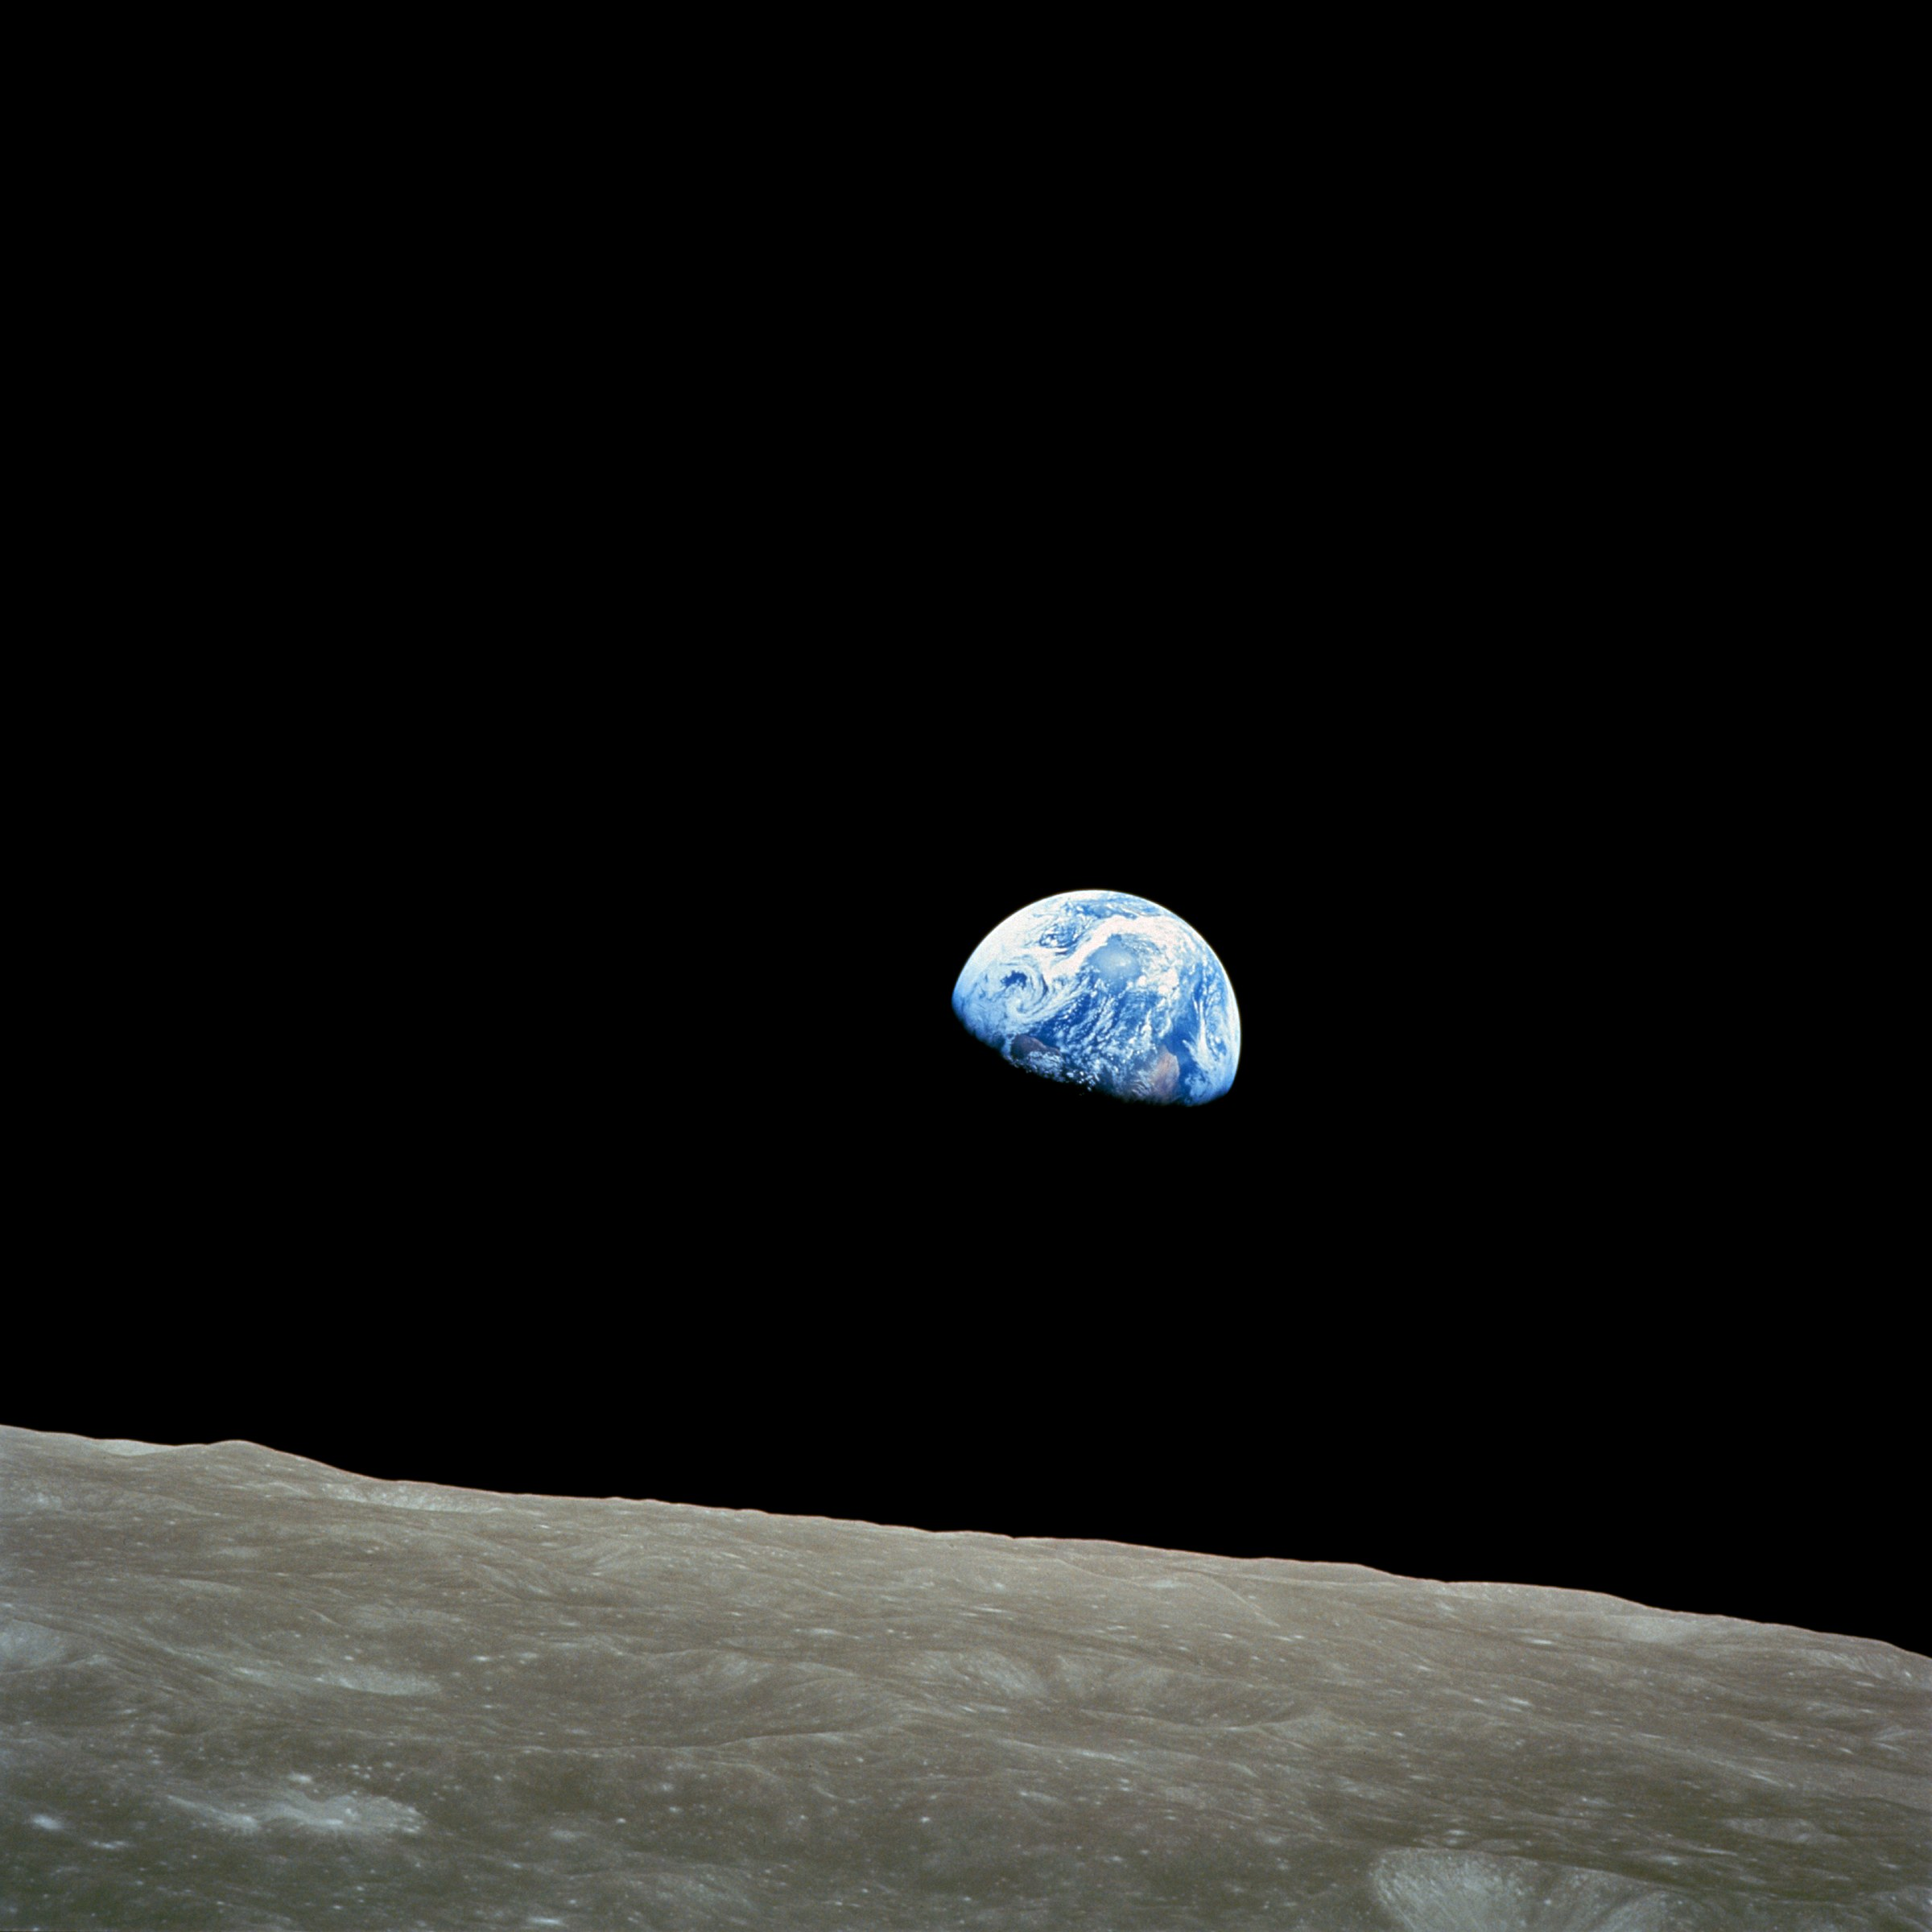
\includegraphics[width=0.95\textwidth]{img/earthrise.jpg}
  \caption{The iconic “Earthrise” photograph taken by astronaut William Anders during the Apollo 8 mission in 1968. Source: NASA.}
  \label{fig:earthrise}
\end{figure}

The postwar decades brought rapid technological progress with the development of radar and synthetic aperture radar (SAR), enabling high-resolution imaging independent of daylight or weather. Early rocket experiments in the late 1940s foreshadowed the space age, initiated by the launch of Sputnik in 1957. NASA's TIROS-1 satellite (1960) delivered the first global meteorological observations, while the launch of Landsat-1 in 1972 introduced systematic multispectral Earth observation, a program that continues today as the longest-running record of land surface change \cite{book_Physics_Techniques_RS,book_Satellite_RS}.

A symbolic milestone came with the Apollo 8 mission in 1968, when astronaut William Anders captured the famous Earthrise photograph, showing Earth rising above the lunar horizon (see Figure \ref{fig:earthrise}). This image not only had profound cultural, philosophical, and scientific impact but also highlighted the scientific value of spaceborne Earth observation.

Since the 1980s, remote sensing has expanded through international efforts such as SPOT (France, 1986), MOS-1 (Japan, 1987), and IRS-1 (India, 1988). The European Space Agency (ESA) \footnote{https://www.esa.int/} launched its first radar satellite, ERS-1, in 1991, and a second with comparable specifications in 1995. The 1990s and 2000s saw the rise of commercial satellites like IKONOS and QuickBird, offering very high-resolution imagery. Today, constellations of small satellites operated by private companies provide near-daily global coverage at meter-scale resolution. These advances—driven by improvements in optics, sensors, data transmission, and digital processing—have transformed remote sensing into a cornerstone of Earth system science, environmental monitoring, disaster response, and planetary exploration \cite{book_Satellite_RS}.

A summary of major milestones in the historical development of remote sensing platforms, from early balloon photography to modern satellite constellations, is illustrated in Figure~\ref{fig:RS_timeline}.

\begin{figure}[H]
  \centering
  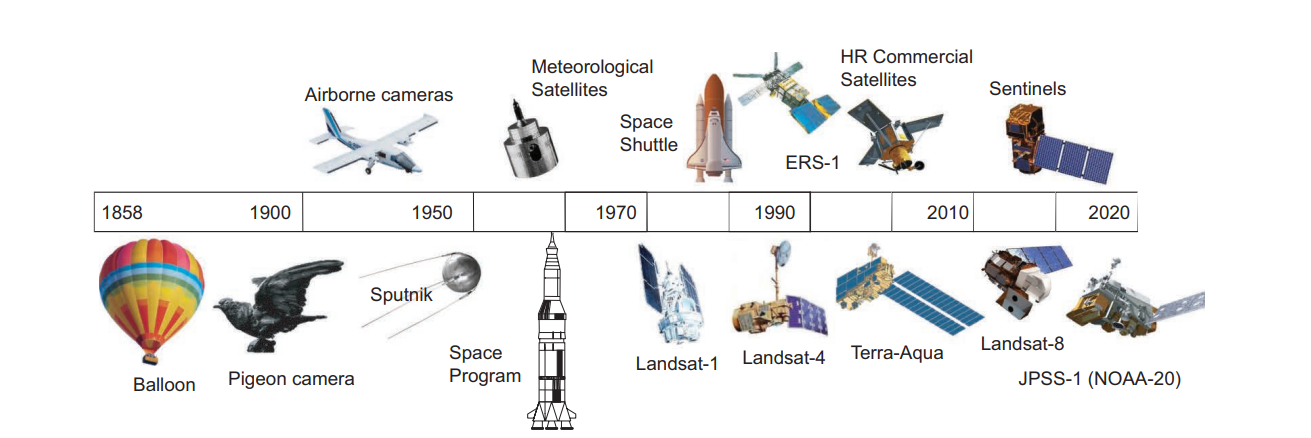
\includegraphics[width=\textwidth]{img/RS_timeline.png}
  \caption{Timeline of remote sensing platform development, from early airborne cameras to modern Earth observation satellites. Adapted from \cite{book_Satellite_RS}.}
  \label{fig:RS_timeline}
\end{figure}


\section{Copernicus: Europe's eyes on Earth}
Copernicus, known as the most ambitious Earth observation programme, is the Earth observation component of the European Union's Space Programme.
It is funded, coordinated, and managed by the European Commission in cooperation with partners such as the European Space Agency (ESA) and the European Organisation for the Exploitation of Meteorological Satellites (EUMETSAT)\footnote{https://www.eumetsat.int/}. The programme was named after the European scientist and observer Nicolaus Copernicus\footnote{https://www.biography.com/scientists/nicolaus-copernicus}. It integrates satellite and in situ observations (e.g., ground stations, airborne and seaborne instruments) to provide reliable, up-to-date information. Its services cover six domains: land, marine, atmosphere, emergency management, security, and climate change. 

The Copernicus Space Component features a new family of dedicated satellites,
called Sentinels, depicted in Figure \ref{fig:sentinels}, specifically designed for the operational needs of the Copernicus programme. 

\begin{figure}[H]
  \centering
  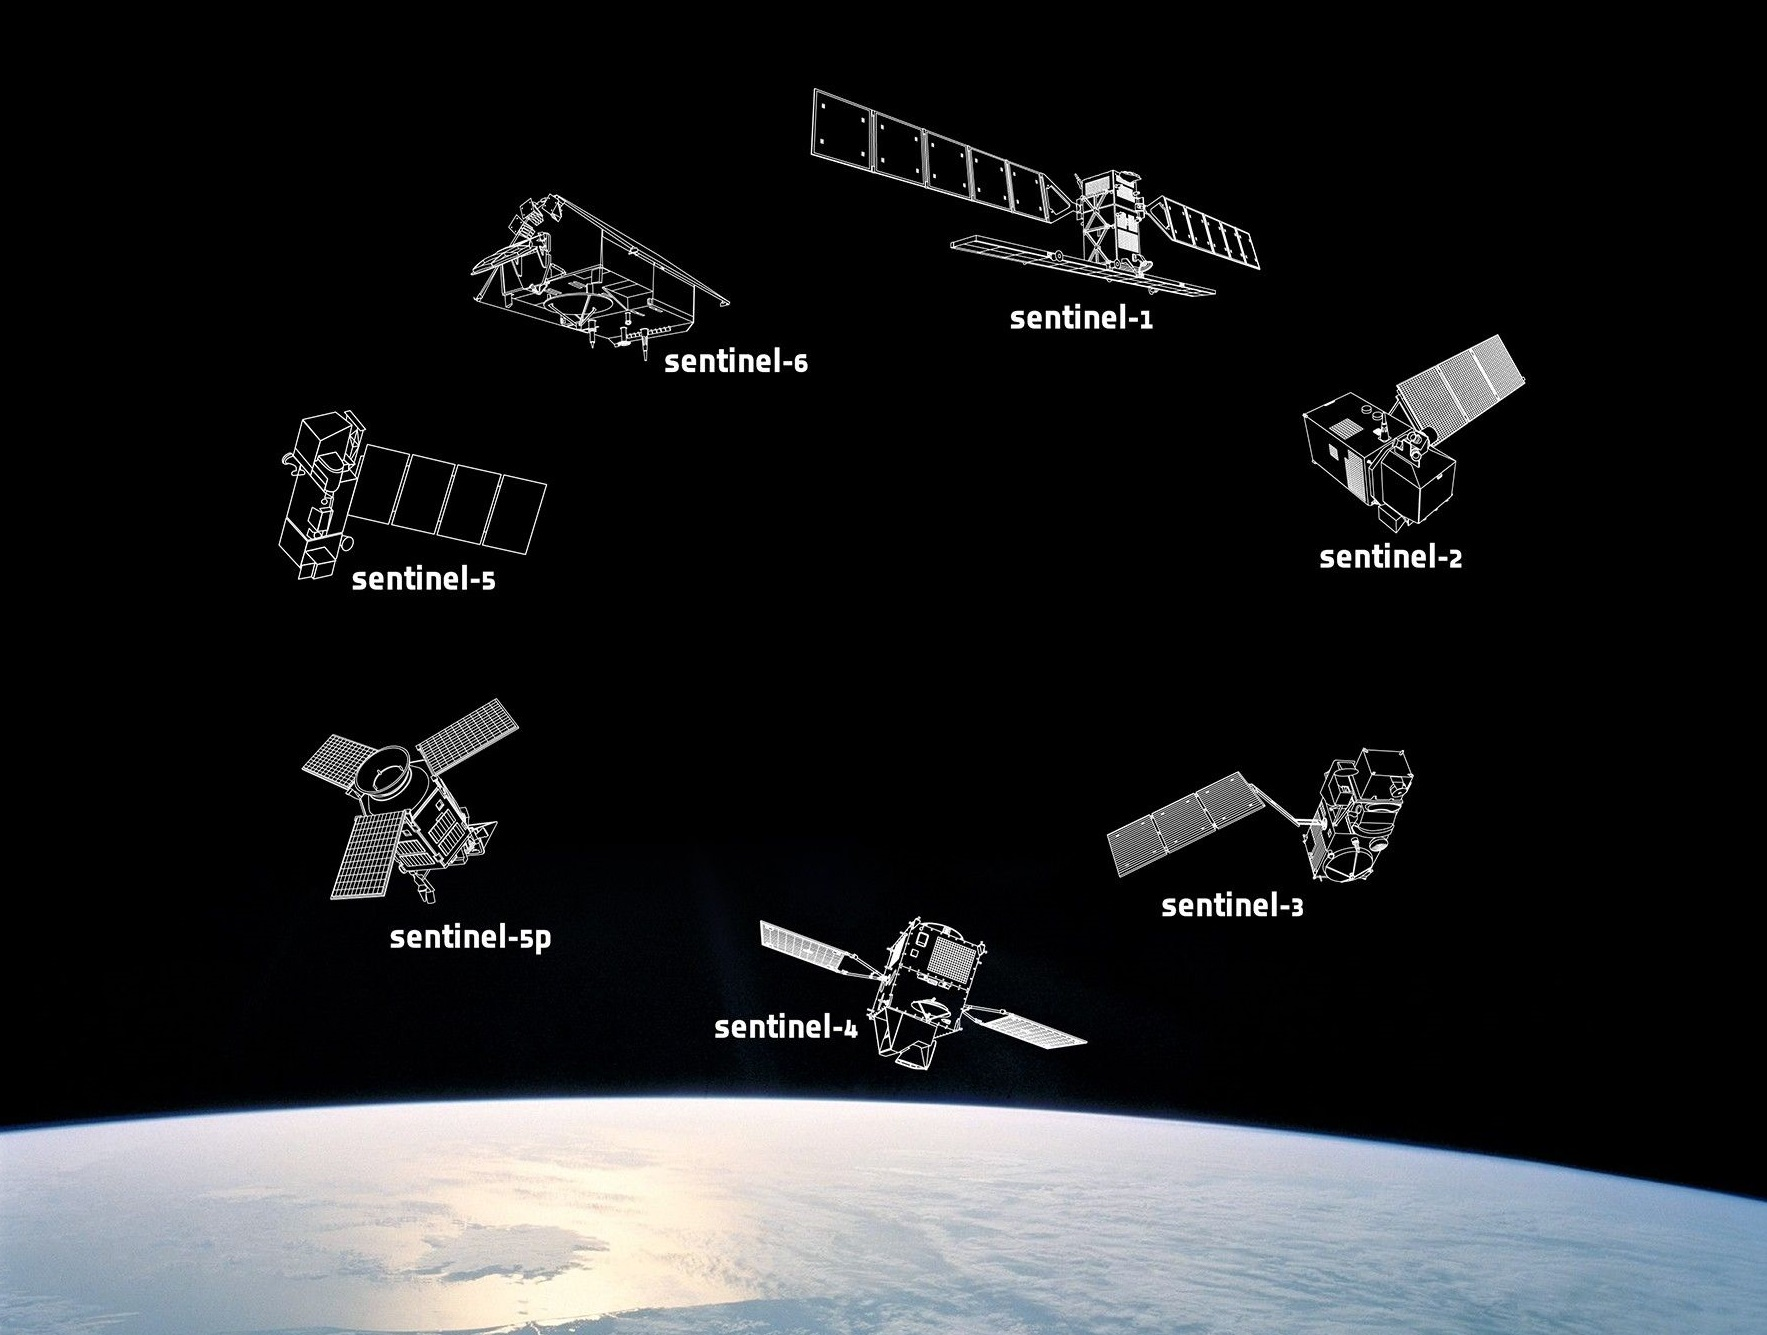
\includegraphics[width=0.95\textwidth]{img/sentinels.png}
  \caption{An artist's impression of the Copernicus Sentinel Missions. Source: ESA.}
  \label{fig:sentinels}
\end{figure}

On 3 April 2014, the deployment of the Copernicus Space Component began with the
launch of the \textsc{Sentinel-1} radar satellite, operating in the C-band and providing all-weather, day-and-night radar imagery. It was followed by its radar successors in 2016 and 2024. Its synthetic aperture radar (SAR) instruments are crucial for monitoring land deformation, subsidence, sea-ice dynamics, and emergency situations such as flooding and earthquakes \cite{ESA_Copernicus,ESA_SentinelMissions}.

\textsc{Sentinel-2}, launched in 2015, 2017, and 2024, is designed to deliver high-resolution, multispectral optical images, supporting applications such as agriculture, forestry, land use, disaster management, and climate studies. Its 13 spectral bands enable detailed analysis of vegetation health, water quality, and land cover dynamics \cite{ESA_Copernicus}.

The two \textsc{Sentinel-3} satellites, launched on 16 February 2016 and 25 April 2018, provide data for services relevant to the ocean and land. They carry instruments to measure sea surface topography, sea and land surface temperature, and ocean and land colour, providing essential data for oceanography, marine resource management, and climate monitoring \cite{ESA_SentinelMissions,ESA_Copernicus}.

\textsc{Sentinel-4} is an ultraviolet, visible, and near-infrared spectrometer carried on the Meteosat Third Generation Sounder satellites. Launched on 1 July 2025, it is dedicated to monitoring atmospheric composition and air quality over Europe and parts of North Africa. It provides hourly measurements of key trace gases and aerosols, enabling near-real-time assessments of air pollution, UV radiation, and climate-relevant processes \cite{ESA_Copernicus}.

Launched on 13 October 2017, the \textsc{Sentinel-5P} mission (Sentinel-5 Precursor) is the first Copernicus mission dedicated to monitoring the atmosphere. It provides high spatio-temporal resolution data for air quality, ozone and UV radiation, as well as climate monitoring and forecasting \cite{ESA_SentinelMissions}.

\textsc{Sentinel-6} is dedicated to high-precision ocean monitoring, focusing on sea surface topography. It continues the long-term record of satellite altimetry, measuring global sea level rise and ocean circulation patterns. These data are critical for climate change research, weather forecasting, and operational oceanography. Sentinel-6 was launched on 21 November 2020 \cite{ESA_SentinelMissions}. 

Looking into the future, six Sentinel Expansion missions will join the fleet. These include, among others, the Hyperspectral Imaging Mission, the Polar Ice and Snow Topography Altimeter, and the Anthropogenic Carbon Dioxide Monitoring mission \cite{ESA_Copernicus}.

Since the focus of this work is on SAR and Optical data, only Sentinel-1 and 2 will be discussed in details in the next sections. 
\subsection{Sentinel-1}
The following description is based on the official SentiWiki resource provided by the European Space Agency \cite{sentiwiki}. 

Sentinel-1, launched on 3 April 2014, constitutes the radar component of the European Copernicus Programme. The mission is designed as a constellation of two sun-synchronous, near-polar orbiting satellites in the same orbital plane, separated by 180° in phase. Equipped with C-band synthetic aperture radar (SAR) operating at 5.4~GHz, Sentinel-1 provides continuous, all-weather, day-and-night imaging capability. Sentinel-1A was followed by Sentinel-1B in 2016, which ceased operations after an anomaly in 2021 and was subsequently replaced by Sentinel-1C in 2024.  

The SAR instrument actively transmits microwave signals towards the Earth and records the backscattered response. Both amplitude and phase are preserved, enabling the reconstruction of high-resolution images. Polarisation diversity further enhances information extraction, as different surfaces exhibit characteristic scattering signatures, supporting classification and retrieval of geophysical parameters.  

Sentinel-1 operates in four exclusive acquisition modes: Stripmap (SM), Interferometric Wide Swath (IW), Extra-Wide Swath (EW), and Wave (WV). These modes achieve spatial resolutions down to 5~m and swath widths of up to 400~km. The system supports single (HH or VV) and dual (HH+HV or VV+VH) polarisation. While SM, IW, and EW modes allow a duty cycle of up to 30 minutes per orbit, WV mode extends this to 75 minutes. Over land, IW mode with VV+VH polarisation is the primary operational configuration, balancing revisit performance, service requirements, and the creation of a consistent long-term archive. For open-ocean observations, WV mode with VV polarisation is predominantly employed, while EW mode is mainly used for sea-ice monitoring and maritime surveillance in high-latitude regions. SM mode is activated only for small islands or in response to emergencies. Across all modes, products are provided at multiple processing levels, from raw SAR data (Level-0) to geophysical ocean products (Level-2 OCN).  

The revisit capabilities of Sentinel-1 are particularly notable. In IW mode, a single satellite can achieve global coverage every 12 days, while the two-satellite constellation reduces the repeat cycle to six days, completing 175 orbits per cycle. These systematic observations, combined with advanced interferometric capabilities, enable the precise detection of land subsidence, structural deformation, and ground movements that are otherwise imperceptible. Such data are invaluable for urban planning, geohazard monitoring, and applications in mining, geology, and risk assessment for infrastructure and natural hazards \cite{sentiwiki}.  

\subsection{Sentinel-2}
The following description is based on the official SentiWiki resource provided by the European Space Agency \cite{sentiwiki}. 

Sentinel-2 is the optical imaging mission of the Copernicus Programme, designed to provide systematic, high-resolution observations over land and coastal regions. The mission consists of a constellation of two sun-synchronous satellites in the same orbital plane, phased 180° apart, ensuring global coverage with a revisit frequency of five days at the Equator. Sentinel-2A was launched in 2015, followed by Sentinel-2B in 2017 and Sentinel-2C in September 2024, the latter ensuring mission continuity as Sentinel-2A approaches the end of its operational lifetime.  

Each satellite carries a single payload: the Multi-Spectral Instrument (MSI). This passive optical sensor collects sunlight reflected from the Earth’s surface, splitting the incoming radiation into two focal plane assemblies: one covering the visible and near-infrared (VNIR) and the other the shortwave infrared (SWIR). The instrument has a swath width of 290~km, which is considerably wider than comparable missions such as Landsat 5/7 (185~km) or SPOT-5 (120~km).  

The MSI samples 13 spectral bands at three spatial resolutions: four bands at 10~m (Blue, Green, Red, and Near-Infrared), six bands at 20~m (red-edge and SWIR), and three bands at 60~m (aerosol, water vapour, and cirrus). These bands span the VNIR to SWIR regions of the electromagnetic spectrum and are tailored to applications including vegetation and crop monitoring, land cover mapping, water quality assessment, snow and ice monitoring, cloud screening, and atmospheric correction. An overview of the spectral bands is provided in Table~\ref{tab:sentinel2_bands}.  

\begin{table}[h]
\centering
\caption{Sentinel-2 MSI spectral bands with central wavelength and spatial resolution \cite{sentiwiki}.}
\label{tab:sentinel2_bands}
\begin{tabular}{@{}lll@{}}
\toprule
\textbf{Band} & \textbf{Central Wavelength [nm]} & \textbf{Resolution [m]} \\ \midrule
B1  & 443  (Aerosols)                & 60 \\
B2  & 490  (Blue)                    & 10 \\
B3  & 560  (Green)                   & 10 \\
B4  & 665  (Red)                     & 10 \\
B5  & 705  (Red edge)                & 20 \\
B6  & 740  (Red edge)                & 20 \\
B7  & 783  (Red edge)                & 20 \\
B8  & 842  (NIR)                     & 10 \\
B8a & 865  (Red edge)                & 20 \\
B9  & 945  (Water vapour)            & 60 \\
B10 & 1375 (Cirrus)                  & 60 \\
B11 & 1610 (SWIR)                    & 20 \\
B12 & 2190 (SWIR)                    & 20 \\ \bottomrule
\end{tabular}
\end{table}

Sentinel-2 imagery is systematically and freely available, supporting several Copernicus services. The Copernicus Land Monitoring Service (CLMS) employs Sentinel-2 for land cover and forest mapping, crop monitoring, ecosystem assessment, and climate change adaptation. The Copernicus Marine Environment Monitoring Service (CMEMS) relies on Sentinel-2 to derive products such as turbidity, chlorophyll, suspended particulate matter, bathymetry, and ice analysis. The Copernicus Emergency Management Service (CEMS) uses Sentinel-2 extensively in disaster response, particularly for rapid mapping of floods, fires, and earthquakes. By enabling systematic, frequent, and global observations, Sentinel-2 has become a cornerstone of Copernicus services, supporting environmental monitoring, resource management, and disaster response worldwide \cite{sentiwiki}.  

Together, Sentinel-1 and Sentinel-2 provide complementary SAR and optical observations, which form the basis of this thesis aiming to translate SAR imagery into its optical counterpart.

\section{Cloud Removal}
As briefly mentioned in the sections above, optical remote sensing imagery, such as Sentinel-2 products, represents a key source of Earth observation data. Compared to SAR observations, multispectral images contain rich spectral information and are readily interpretable by the human eye. Such data play an essential role in a wide range of applications, including environmental monitoring, resource exploration, and disaster assessment. While the quality and quantity of satellite observations have dramatically increased in recent years, one common problem persists for optical remote sensing imagery: \textbf{cloud cover}.

Based on findings from the International Satellite Cloud Climatology Project (ISCCP), average global cloud cover surpasses 66\% \cite{dl_cloud_detection_survey,aCGAN_fuse_sar_MS,CR_SEN2_dRNN}, with 55\% over land surface alone \cite{CR_SEN2_dRNN}, preventing optical satellites from acquiring valuable information about the Earth's surface due to the frequent presence of clouds in the imagery. In contrast to SAR instruments, optical sensors cannot penetrate clouds, resulting in considerable data gaps in both the spatial and temporal domains. For applications requiring consistent time series, e.g., agricultural monitoring, or where a specific scene must be observed at a given time, e.g., disaster monitoring, cloud cover represents a serious limitation \cite{CR_SEN2_dRNN}. The diversity of clouds —including thin and thick clouds as well as haze— together with the wide range of occlusion scenarios and their uneven distribution, poses an additional challenge for image reconstruction and the generalizability of cloud removal techniques\cite{CR_Advances_Review_ORS}.

Consequently, removing clouds and obtaining cloud-free optical data to retrieve surface information is both of theoretical importance and practical necessity. Cloud removal in optical remote sensing imagery aims to mitigate or eliminate the influence of clouds, thereby revealing more accurate and complete surface details \cite{CR_Advances_Review_ORS}. In response to this challenge, a wide range of approaches have been proposed. These methods can broadly be divided into three categories: (i) single-image methods, (ii) multimodal-based methods, and (iii) multitemporal-based methods \cite{CR_Advances_Review_ORS}. The main categories and their characteristics are summarized below

\begin{enumerate}[label=(\Alph*)]
  \item \textbf{Single-image methods:} Constrained by the limited acquisition capabilities of early remote sensing data, single-image cloud removal techniques attempt to restore surface information using only the cloudy optical image. Classical approaches employ statistical and physical models such as spatial similarity, frequency filtering, or atmospheric scattering models. For example, Zhang et al. \cite{single_variation} proposed the \emph{Haze Optimized Transformation (HOT)}, which detects and compensates for thin cloud and haze contamination in Landsat images by exploiting the spectral correlation of clear-sky bands and quantifying deviations caused by haze. Similarly, He et al. \cite{single_haze_removal_dark_prior} introduced the \emph{dark channel prior}, a widely used statistical prior that estimates haze thickness from local image patches to recover clear radiance, later adapted for thin cloud removal in optical remote sensing. With the advent of deep learning, CNNs, U-Nets, and GAN-based architectures have been applied to learn the mapping from cloudy to cloud-free domains, sometimes extended with unpaired learning schemes like CycleGANs. Notably, U-Net-based methods have been widely used for their encoder-decoder structures, while CycleGAN approaches exploit cycle consistency loss to preserve colors and textures during cloudy-to-clear translation. While these methods demonstrate effectiveness for thin or semi-transparent clouds, their reliance on information present in a single image limits their applicability to dense cloud cover. In such cases, they cannot reliably reconstruct surface features, which has motivated the integration of external data sources such as SAR imagery \cite{CR_Advances_Review_ORS}.

  \item \textbf{Multimodal-based methods:} Multimodal strategies explicitly integrate auxiliary data from other sensors to improve optical image restoration. Multispectral-based methods exploit the differential sensitivity of spectral bands, but the most notable progress has been achieved by fusing synthetic aperture radar (SAR) with optical imagery. A representative work is Meraner et al. \cite{CR_SEN2_dRNN}, who proposed the DSen2-CR framework, a deep residual network that combines Sentinel-1 and Sentinel-2 data to improve reconstructions under thick cloud cover and preserve spectral fidelity. Likewise, Grohnfeldt et al. \cite{A_cGAN_fuse_sar_MS_CR} demonstrated the potential of conditional GANs (cGANs) to fuse SAR and multispectral data for cloud removal, highlighting the advantages of adversarial training in capturing nonlinear relationships between modalities. More recently, Xu et al. \cite{GLF_CR} presented the GLF-CR model, which applies a global–local fusion strategy to better exploit SAR features for cloud removal. SAR-to-optical image translation has thus emerged as a powerful paradigm in this context, as SAR penetrates cloud layers and provides structural information that can guide optical reconstruction. A wide range of approaches have been proposed, including CNN-based fusion, cGANs, and CycleGAN-style frameworks, which either translate SAR features into optical-like imagery or combine them with partially corrupted optical inputs. These methods have proven especially effective in recovering surface information under dense and persistent cloud conditions, although challenges remain in terms of data registration, modality differences, and SAR-induced speckle noise.

  \item \textbf{Multitemporal-based methods:} Multitemporal approaches leverage repeated acquisitions of the same location at different times to fill in cloud-covered areas. \textit{Non-blind} methods use cloud masks to guide restoration, whereas \textit{blind} methods directly infer cloud-free information from temporal sequences. A classical example is the work of Xu et al. \cite{CR_spars_repre_MT_dict_L}, who proposed a sparse representation framework with multitemporal dictionary learning (MDL) that learns dictionaries from both cloudy and clear images, effectively reconstructing areas obscured by thin and thick clouds without requiring explicit cloud masks. More recently, Ebel et al. \cite{UnCRtainTS} introduced UnCRtainTS, an attention-based deep learning model that not only reconstructs cloud-free images from Sentinel-1/2 time series but also quantifies pixel-wise uncertainty, providing reliability measures alongside the reconstructed outputs. Techniques therefore range from traditional model-driven approaches, such as low-rank tensor decomposition and sparse representation, to data-driven deep learning frameworks that learn spatio-temporal mappings. Recent research has also begun to combine multitemporal optical data with SAR, creating hybrid SAR–optical time series methods that enhance robustness under persistent cloud cover and enable more accurate SAR-to-optical translation. Although highly effective for dense cloud removal, these approaches face challenges such as geometric misalignment, temporal variability in land cover, and the need for large, paired training datasets \cite{CR_Advances_Review_ORS}.

\end{enumerate}

As shown in Table~\ref{tab:cloud_removal_categories}, research on cloud removal has been uneven across categories. Single-image methods have been the most extensively studied due to their simplicity and minimal data requirements, though their effectiveness is limited under dense clouds. Multimodal approaches, particularly SAR–optical fusion, have gained significant traction in recent years and are currently the most active research direction. By contrast, multitemporal methods, while highly effective in principle, are less frequently explored because of the challenges in acquiring consistent, well-aligned time series data.

\begin{table}[ht]
\centering
\caption{Summary of cloud removal categories, their advantages and limitations \cite{CR_Advances_Review_ORS, sar_2_opt_CGAN_survey_taxonomy}.}
\label{tab:cloud_removal_categories}
\begin{adjustbox}{max width=\textwidth, keepaspectratio=false}
\begin{tabular}{p{2.5cm} p{6cm} p{6cm} p{3cm}}
\toprule
\textbf{Category} & \textbf{Advantages} & \textbf{Limitations} & \textbf{Representative literature} \\
\midrule
\textbf{Single-image} & 
\begin{itemize}[nosep,leftmargin=*]
  \item No auxiliary data required (cost- and time-efficient).
  \item Effective for thin or semi-transparent clouds.
  \item Straightforward implementation with statistical/physical models or deep learning.
\end{itemize} &
\begin{itemize}[nosep,leftmargin=*]
  \item Ineffective for dense or opaque clouds.
  \item Often introduces artifacts or color distortions.
  \item Deep learning requires large paired datasets, which are difficult to obtain.
\end{itemize} &
\cite{single_variation} \cite{single_haze_removal_dark_prior} \cite{single_artifact_free_CR_GAN} \cite{single_thin_CR_ORS_GAN_phys} \cite{single_multi_DR_CR} \cite{single_CR_DLM_matting} \cite{single_AGLC_GAN} \cite{single_PNBT_CR} \cite{single_CGAN_scattering_martian} \\
\midrule
\textbf{Multimodal} &
\begin{itemize}[nosep,leftmargin=*]
  \item Integrates complementary information from other sensors.
  \item Multispectral bands provide spectral redundancy.
  \item SAR–optical fusion enables SAR-to-optical translation, penetrating cloud layers.
  \item Suitable for both thin and thick clouds.
\end{itemize} &
\begin{itemize}[nosep,leftmargin=*]
  \item Requires accurate registration of heterogeneous data.
  \item SAR data introduces speckle noise.
  \item High computational complexity and preprocessing effort.
\end{itemize} &
\cite{A_cGAN_fuse_sar_MS_CR} \cite{sar2opt_cGAN_Optim_oppr_limits} \cite{syn_ms_sar_opt_MT_cGAN} \cite{CR_SEN2_dRNN} \cite{GAN_gen_synt_MS} \cite{s2o_ViT_cGAN} \cite{CR_RS_GAN_s2o} \cite{s2o_Thermodynamics} \cite{c_diffusion_s2o} \cite{s2o_color_super_diff} \cite{S2MS_GAN} \cite{SAR_DeCR} \\
\midrule
\textbf{Multitemporal} &
\begin{itemize}[nosep,leftmargin=*]
  \item Exploits temporal redundancy to reconstruct cloudy regions.
  \item Effective for dense and extensive cloud cover.
  \item Deep learning models can capture spatio-temporal correlations.
  \item Can be extended with SAR–optical time series for improved robustness.
\end{itemize} &
\begin{itemize}[nosep,leftmargin=*]
  \item Sensitive to geometric misalignment and temporal variability.
  \item Requires consistent multitemporal datasets, which may be unavailable.
  \item Landscape or seasonal changes reduce restoration accuracy.
\end{itemize} &
\cite{syn_ms_sar_opt_MT_cGAN} \cite{CR_RS_spati_atten_GAN} \cite{UnCRtainTS} \cite{assessing_MT_cGANS_s2o_crop} \cite{DiffCR} \\
\bottomrule
\end{tabular}
\end{adjustbox}
\end{table}

In summary, cloud removal research spans single-image, multimodal, and multitemporal strategies, each with distinct advantages and limitations, as outlined in Table~\ref{tab:cloud_removal_categories} together with representative literature. Among these, SAR-to-optical image translation has recently emerged as a particularly promising direction, as it leverages the cloud-penetrating capability of SAR while producing optical-like imagery suitable for interpretation and analysis. This thesis builds on this line of research by systematically investigating and advancing SAR-to-optical translation methods for cloud removal.

\section{Generative AI}
\subsection{Pre-GenAI: Classical Approaches}
\subsection{Deep Learning and Computer Vision}
\subsection{Generative Adversarial Networks (GANs)}
\subsection{Diffusion Models}
\subsection{Vision Transformer}
\subsection{Vision Mamba}

\section{Application and Relevance to KIWA}



% \chapter{Literature Review}
Cloud contamination in optical remote sensing imagery hinders continuous Earth observation, limiting applications such as crop monitoring and land cover classification. Synthetic Aperture Radar (SAR) systems can penetrate clouds, enabling data acquisition in all weather conditions. This capability makes SAR data valuable for filling gaps in optical time series, driving research into SAR–optical fusion and SAR-to-optical image translation for cloud removal.

Early methods leveraged traditional signal processing techniques. Huang et al.~\cite{huang2015} introduced sparse representation-based cloud removal using SAR data, which Xu et al.~\cite{xu2016} extended via multi-temporal dictionary learning. These approaches, however, struggled under heavy cloud cover or highly dynamic surface changes.

Deep learning transformed the field. The foundational GAN framework was introduced by Goodfellow et al.~\cite{goodfellow2014}, and Mirza \& Osindero~\cite{mirza2014} extended it to conditional GANs (cGANs), ideal for image-to-image tasks like SAR-to-optical translation. Enomoto et al.~\cite{enomoto2017} applied cGANs for cloud removal using NIR input, though dense clouds remained problematic. To address this, Grohnfeldt et al.~\cite{grohnfeldt2018} proposed SAR-Opt-cGAN to fuse Sentinel-1 SAR and Sentinel-2 optical data; Bermudez et al.~\cite{bermudez2018} explored cGAN-based SAR-to-optical synthesis for crop classification. The SEN1-2~\cite{schmitt2018} and SEN12MS~\cite{schmitt2019} datasets were pivotal for training deep models.

Advancements continued with Fuentes Reyes et al.~\cite{fuentes2019} on cGAN optimization, Wang et al.~\cite{wang2019} with supervised CycleGANs for translation, Meraner et al.~\cite{meraner2020} introducing DSen2-CR networks, Abady et al.~\cite{abady2020} leveraging ProGANs, and Pan~\cite{pan2020} with spatial-attention models. Gao et al.~\cite{gao2020} developed fusion-based GAN approaches for high-resolution images.

Recent models show increasing complexity: Naderi Darbaghshahi et al.~\cite{naderi2021} proposed a two-GAN model with DRIBs, Ebel et al.~\cite{ebel2022} introduced UnCRtainTS with uncertainty prediction, Kwak \& Park~\cite{kwak2024} proposed MTcGANs, and Liu et al.~\cite{liu2024} developed S2MS-GAN.

Diffusion models have found their way into this field: Bai et al.~\cite{bai2023} proposed a conditional diffusion model; Bai et al.~\cite{bai2024} extended it with color supervision; Zou et al.~\cite{zou2023} introduced the efficient DiffCR framework.

Vision Transformers (ViT) also made inroads: Dosovitskiy et al.~\cite{dosovitskiy2020} introduced the original ViT, while Park et al.~\cite{park2025} integrated multiscale ViT blocks into a cGAN for SAR-optical tasks. However, ViTs are computationally intensive.

Alternatives emerged via SSMs: Gu \& Dao~\cite{gu2023} introduced Mamba—an efficient, linear-complexity sequence model. U-Mamba~\cite{umamba2024} adapted this into a U-Net architecture, and Swin-UMamba~\cite{swinumamba2024} enhanced it further using ImageNet pretraining. Swin-UNet~\cite{swinunet2023} remains a benchmark transformer-based segmentation model. This thesis explores applying U-Mamba (and its Swin-UMamba variant) to SAR-to-optical translation and cloud removal.


\chapter{Methodology}

\section{Datasets}
\subsection{SEN12-MS}
This thesis relies exclusively on the SEN12MS dataset~\cite{sen12ms_2019}, curated by Schmitt et al.. SEN12MS is a large-scale, globally distributed benchmark explicitly designed to advance research in multimodal Earth observation and deep learning. It comprises 180,662 georeferenced image triplets, each consisting of (i) dual-polarized Sentinel-1 synthetic aperture radar (SAR) data in VV and VH polarization ($\sigma^{0}$ backscatter values in decibel scale), (ii) full Sentinel-2 multispectral imagery spanning all 13 bands, and (iii) MODIS land cover maps derived from the MCD12Q1 product and resampled to 10 m resolution. Each triplet is stored as a 256 × 256 pixel GeoTIFF at 10 m ground sampling distance, corresponding to a spatial coverage of approximately 2.56 × 2.56 km per patch.

The Sentinel-1 component originates from ground-range-detected (GRD) products acquired in interferometric wide swath (IW) mode. These data were radiometrically calibrated and orthorectified against SRTM or ASTER digital elevation models to ensure accurate geolocation. The Sentinel-2 imagery was curated using a cloud-free mosaicking workflow on Google Earth Engine: within each region of interest (ROI), multiple observations collected during a given meteorological season of 2017 were composited such that cloud-contaminated pixels were systematically excluded. This procedure ensured that every ROI is represented by seasonally consistent, nearly cloud-free multispectral data. Finally, the MODIS land cover maps were used to generate categorical reference layers; however, due to their relatively coarse native resolution (500 m), they are subject to spatial inaccuracies even after upsampling.

\begin{figure}[htbp]
    \centering
    % First row: SAR images
    \begin{subfigure}{0.18\textwidth}
        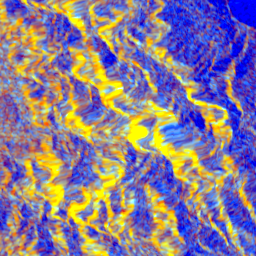
\includegraphics[width=\linewidth]{img/ROIs2017_winter_s1_68_p100.png}
    \end{subfigure}
    \begin{subfigure}{0.18\textwidth}
        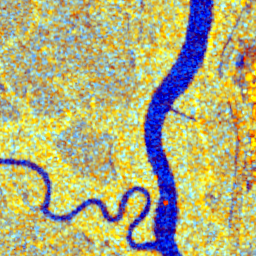
\includegraphics[width=\linewidth]{img/ROIs1970_fall_s1_105_p100.png}
    \end{subfigure}
    \begin{subfigure}{0.18\textwidth}
        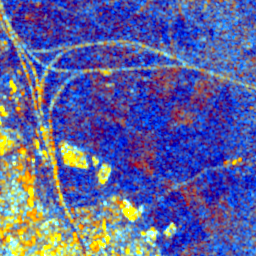
\includegraphics[width=\linewidth]{img/ROIs1970_fall_s1_128_p100.png}
    \end{subfigure}
    \begin{subfigure}{0.18\textwidth}
        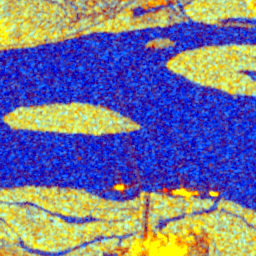
\includegraphics[width=\linewidth]{img/ROIs2017_winter_s1_104_p101.png}
    \end{subfigure}
    \begin{subfigure}{0.18\textwidth}
        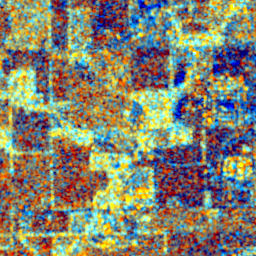
\includegraphics[width=\linewidth]{img/ROIs1970_fall_s1_145_p100.png}
    \end{subfigure}

    \begin{subfigure}{0.18\textwidth}
        \centering
        {\footnotesize \textit{Winter ROI-68-100}}
    \end{subfigure}
    \begin{subfigure}{0.18\textwidth}
        \centering
        {\footnotesize \textit{Fall ROI-105-100}}
    \end{subfigure}
    \begin{subfigure}{0.18\textwidth}
        \centering
        {\footnotesize \textit{Fall ROI-128-100}}
    \end{subfigure}
    \begin{subfigure}{0.18\textwidth}
        \centering
        {\footnotesize \textit{Winter ROI-104-101}}
    \end{subfigure}
    \begin{subfigure}{0.18\textwidth}
        \centering
        {\footnotesize \textit{Fall ROI-145-100}}
    \end{subfigure}
    
    \vspace{0.5em}

    % Second row: MS images
    \begin{subfigure}{0.18\textwidth}
        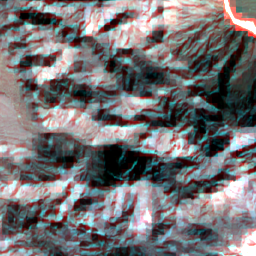
\includegraphics[width=\linewidth]{img/ROIs2017_winter_s2_68_p100.png}
    \end{subfigure}
    \begin{subfigure}{0.18\textwidth}
        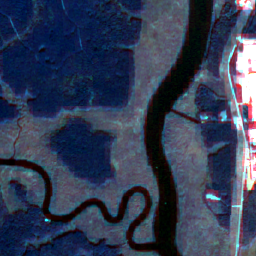
\includegraphics[width=\linewidth]{img/ROIs1970_fall_s2_105_p100.png}
    \end{subfigure}
    \begin{subfigure}{0.18\textwidth}
        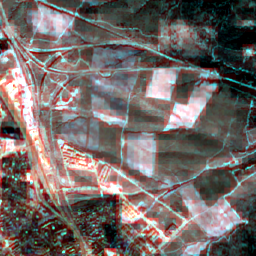
\includegraphics[width=\linewidth]{img/ROIs1970_fall_s2_128_p100.png}
    \end{subfigure}
    \begin{subfigure}{0.18\textwidth}
        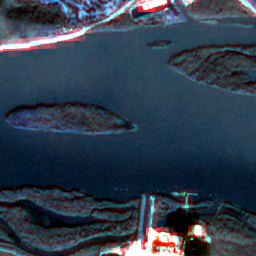
\includegraphics[width=\linewidth]{img/ROIs2017_winter_s2_104_p101.png}
    \end{subfigure}
    \begin{subfigure}{0.18\textwidth}
        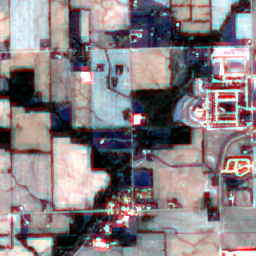
\includegraphics[width=\linewidth]{img/ROIs1970_fall_s2_145_p100.png}
    \end{subfigure}

    \caption{Sample pairs from the SEN12MS dataset. Top row: Sentinel-1 SAR patches (R: VV, G: VH, B: VV/VH). Bottom row: corresponding Sentinel-2 multispectral patches (only RGB bands).}
    \label{fig:sen12ms_pairs}
\end{figure}


Importantly, all triplets underwent manual verification by a remote sensing expert. This revision step ensured that each patch is free from major artifacts, severe registration errors, or residual cloud contamination, thereby guaranteeing the dataset’s quality and usability for machine learning tasks.

The ROIs were sampled globally across all inhabited continents and four meteorological seasons of 2017 to maximize spatial and temporal diversity. Nevertheless, it should be noted that the ROI selection was not purely random. In practice, locations were chosen to avoid large homogeneous areas such as deserts or oceans and to ensure inclusion of diverse land cover classes. While this design improves the dataset’s representativeness for a wide range of applications, it may introduce a bias toward heterogeneous landscapes and thus does not fully capture the true global distribution of land cover types.

For the purpose of this thesis, which addresses translation from SAR to multispectral optical imagery, only the Sentinel-1 and Sentinel-2 modalities are employed. The MODIS land cover products included in SEN12MS are disregarded, as they are not directly relevant to the translation task.

\subsection{SEN12 datasets Family}
SEN12MS is part of a broader line of datasets developed to foster multimodal remote sensing research. Its direct predecessor, SEN1-2~\cite{sen12_2018}, curated by the same research group, contained approximately 282,000 paired patches of Sentinel-1 VV data and Sentinel-2 RGB composites. While groundbreaking in bridging SAR and optical domains, SEN1-2 lacked georeferencing, full spectral coverage, and multi-polarization SAR, limiting its applicability for remote sensing research beyond proof-of-concept image translation.

SEN12MS addressed these limitations by introducing full multispectral coverage, dual-polarized SAR, geocoded products, and auxiliary land cover labels, making it a comprehensive multimodal benchmark. Building upon this foundation, the dataset family has since been extended. SEN12MS-CR~\cite{sen12ms-cr_2021} added temporally matched cloudy and cloud-free Sentinel-2 imagery alongside Sentinel-1 data, enabling the development and benchmarking of cloud removal methods under realistic atmospheric conditions. Subsequently, SEN12MS-CR-TS~\cite{sen12ms-cr-ts_2022} expanded the concept into the temporal domain, providing year-long multimodal time series with 30 co-registered Sentinel-1 and Sentinel-2 acquisitions per ROI. This evolution reflects a progression from simplified SAR–optical pairs, to globally diverse multimodal data, to temporally rich resources designed for time-series analysis and robust cloud removal.

A comparsion of these different datasets is provided in Table~\ref{tab:sen12_datasets}. In this thesis, however, the focus remains on the SEN12MS dataset, leveraging its multimodal SAR and multispectral imagery for the study of SAR-to-optical translation.

% in preamble:
% \usepackage{array,booktabs,adjustbox}
% ragged-right p-columns
\newcolumntype{P}[1]{>{\raggedright\arraybackslash}p{#1}}

\begin{table}[!h]
    \centering
    \caption{Comparison of datasets in the SEN12 family.}
    \label{tab:sen12_datasets}
    \setlength{\tabcolsep}{4pt} % tighter horizontal padding
    \renewcommand{\arraystretch}{1.15} % a bit more vertical room
    \begin{adjustbox}{max width=\textwidth, keepaspectratio=false}
    \begin{tabular}{P{2.6cm} P{3.4cm} P{3.4cm} P{3.6cm} P{3.6cm}}
        \toprule
        \textbf{Aspect} &
        \textbf{SEN1-2}~\cite{sen12_2018} &
        \textbf{SEN12MS}~\cite{sen12ms_2019} &
        \textbf{SEN12MS-CR}~\cite{sen12ms-cr_2021} &
        \textbf{SEN12MS-CR-TS}~\cite{sen12ms-cr-ts_2022} \\
        \midrule
        \textbf{Year released} &
        2018 & 2019 & 2021 & 2022 \\
        \addlinespace[6pt]
        \textbf{Main purpose} &
        Proof-of-concept SAR–optical translation &
        Multimodal learning and data fusion &
        Cloud removal with real cloudy/clear pairs &
        Multi-temporal cloud removal (sequence models) \\
        \addlinespace[6pt]
        \textbf{Modalities} &
        S1 (VV), S2 (RGB) &
        S1 (VV,VH), S2 (13 bands), MODIS LULC &
        S1 (VV,VH), S2 (13 bands; cloudy \& cloud-free) &
        S1 (VV,VH), S2 (13 bands; cloudy \& cloud-free time series) \\
        \addlinespace[6pt]
        \textbf{Georeferencing} &
        Not georeferenced &
        Fully georeferenced &
        Fully georeferenced &
        Fully georeferenced \\
        \addlinespace[6pt]
        \textbf{Spatial sampling} &
        Global patch pairs (282k) &
        180,662 patch triplets across 2017 seasons &
        169 ROIs; $>$100k patch triplets &
        53 ROIs; 30 time steps per ROI \\
        \addlinespace[6pt]
        \textbf{Temporal coverage} &
        Single time-point &
        Seasonal (2017) &
        Seasonal with paired cloudy/clear &
        Year-long time series (2018) \\
        \addlinespace[6pt]
        \textbf{Patch size} &
        $256\times256$ px &
        $256\times256$ px &
        $256\times256$ px &
        $256\times256$ px \\
        \addlinespace[6pt]
        \textbf{Notable limitations} &
        RGB only; VV only; no geocoding &
        MODIS labels are coarse (upsampled) &
        Mono-temporal pairs (no full time series) &
        Fewer ROIs; large storage ($\sim$2\,TB) \\
        \bottomrule
    \end{tabular}
    \end{adjustbox}
\end{table}


\section{Models}
\subsection{Pix2Pix Model}
The image translation task in this thesis is addressed using the \textit{pix2pix} framework, introduced by Isola et al.~\cite{pix2pix_2018}. Pix2pix is based on the concept of \textit{conditional generative adversarial networks} (cGANs), which extend the original GAN formulation by conditioning both the generator and discriminator on an input image. In this setup, the generator $G$ learns to map an input image $x$ to an output image $y$, while the discriminator $D$ learns to distinguish between real image pairs $\{x, y\}$ and synthesized pairs $\{x, G(x)\}$. This adversarial objective enforces that generated outputs are not only realistic but also structurally consistent with the given input.

Formally, the cGAN loss is defined as:
\begin{equation}
    \mathcal{L}_{cGAN}(G,D) = \mathbb{E}_{x,y}[\log D(x,y)] + \mathbb{E}_{x}[\log(1 - D(x,G(x)))].
\end{equation}
To encourage fidelity to the target image, the adversarial loss is combined with an $\ell_{1}$ reconstruction loss:
\begin{equation}
    \mathcal{L}_{\ell_1}(G) = \mathbb{E}_{x,y}[\|y - G(x)\|_1].
\end{equation}
The final objective is then:
\begin{equation}
    G^* = \arg \min_G \max_D \; \mathcal{L}_{cGAN}(G,D) + \lambda \mathcal{L}_{\ell_1}(G),
\end{equation}
where $\lambda$ balances realism and reconstruction accuracy. Following Isola et al., $\lambda = 100$ is typically used.

\paragraph{Generator architecture.}  
The generator is implemented as a \textit{U-Net} encoder–decoder~\cite{U-net_2015}. Unlike a plain encoder–decoder, U-Net introduces skip connections between corresponding downsampling and upsampling layers, allowing low-level spatial details from the input to directly propagate to the output. This design is particularly effective in tasks where the input and output share spatial structures, as in SAR-to-optical translation.

\paragraph{Discriminator architecture.}  
The discriminator follows a \textit{PatchGAN} design, which classifies local $N \times N$ patches of an image as real or fake instead of operating on the entire image~\cite{pix2pix_2018}. This approach emphasizes high-frequency correctness and enforces local realism, while the $\ell_1$ loss ensures global structural coherence. The original work demonstrates that a patch size of $70 \times 70$ provides a good trade-off between quality and efficiency.

\paragraph{Optimization.}  
Training alternates between updating $D$ to improve its ability to classify real versus fake pairs, and updating $G$ to fool $D$ while minimizing the $\ell_1$ distance to the target. The Adam optimizer~\cite{adam_optimizer_2017} with learning rate $2 \times 10^{-4}$ and momentum parameters $\beta_1=0.5$, $\beta_2=0.999$ is typically employed. Dropout is used at both training and inference time to introduce stochasticity, though in practice outputs remain largely deterministic.

\paragraph{Relevance to this work.}  
The pix2pix framework provides a principled and general-purpose solution for image-to-image translation tasks. In the context of this thesis, it is employed to learn mappings from Sentinel-1 SAR inputs to Sentinel-2 multispectral optical outputs. The combination of adversarial and reconstruction losses, together with the U-Net generator and PatchGAN discriminator, makes pix2pix particularly suitable for producing sharp, realistic, and structurally aligned multispectral predictions.


\section{Evaluation Metrics}
The effectiveness of SAR-to-optical image translation depends not only on the choice of translation models but also on the methods employed for quality assessment. Image Quality Assessment (IQA) serves two key purposes: (i) to objectively evaluate the quality of results produced by different models, and (ii) to guide the optimization of network architectures and algorithms~\cite{quality_assessment_S2OT}.

In~\cite{quality_assessment_S2OT}, five IQA metrics—SSIM, FSIM, MSE, LPIPS, and DISTS—were compared through image restoration experiments to identify suitable measures for SAR-to-optical translation. Their results showed that SSIM, MSE, and LPIPS consistently aligned with human perception, converged reliably, and effectively captured both structural and textural details, whereas FSIM often failed to capture fine details and DISTS exhibited instability. Consequently, SSIM, MSE, and LPIPS were recommended as complementary metrics for pixel-level fidelity, structural similarity, and perceptual quality. Nevertheless, as summarized in Table~\ref{tab:iqa}, SSIM, PSNR, and SAM remain the most widely used indicators in SAR-to-optical translation, fusion, and cloud removal tasks, while LPIPS and MSE appear far less frequently. This distribution is consistent with the findings reported in the literature survey~\cite{sar_2_opt_CGAN_survey_taxonomy}.

\textcolor{red}{TODO: specify which metrics will be used and why}

\begin{table}[h!]
\centering
\begin{tabular}{lll}
\toprule
\textbf{Metric} & \textbf{References} & \textbf{Frequency} \\
\midrule
Structural Similarity Index Measurement (SSIM)~\cite{iqa_ssim}
 & \cite{CR_Advances_Review_ORS, RS_Data_Fusion_GANs_sota, DiffCR, c_diffusion_s2o, s2o_ViT_cGAN, S2MS_GAN, c_guided_fus_s2ot, transfusion_cr, trans_gan_CF, hvt_cgan, msf_gan, diffusion_memory} 
 & 12 \\
Peak Signal-to-Noise Ratio (PSNR)~\cite{iqa_psnr}
 & \cite{CR_Advances_Review_ORS, DiffCR, CR_RS_spati_atten_GAN, s2o_ViT_cGAN, CR_RS_GAN_s2o, S2MS_GAN, c_guided_fus_s2ot, transfusion_cr, trans_gan_CF, hvt_cgan, msf_gan, diffusion_memory} 
 & 12 \\
Spectral Angle Mapper (SAM)~\cite{iqa_sam}
 & \cite{aCGAN_fuse_sar_MS, RS_Data_Fusion_GANs_sota, CR_RS_GAN_s2o, S2MS_GAN, c_guided_fus_s2ot, transfusion_cr, trans_gan_CF, cond_brownian, hvt_cgan, msf_gan} 
 & 11 \\
Fréchet Inception Distance (FID)~\cite{iqa_fid}
 & \cite{DiffCR, c_diffusion_s2o, s2o_ViT_cGAN, cond_brownian, hvt_cgan, msf_gan} 
 & 6 \\
Root Mean Square Error (RMSE) 
 & \cite{aCGAN_fuse_sar_MS, CR_Advances_Review_ORS, RS_Data_Fusion_GANs_sota, CR_RS_GAN_s2o, c_guided_fus_s2ot} 
 & 5 \\
Learned Perceptual Image Patch Similarity (LPIPS)~\cite{iqa_lpips}
 & \cite{CR_Advances_Review_ORS, DiffCR, S2MS_GAN, cond_brownian, diffusion_memory} 
 & 5 \\
Mean Absolute Error (MAE) 
 & \cite{CR_RS_GAN_s2o, c_guided_fus_s2ot} 
 & 2 \\
Mean Square Error (MSE) 
 & \cite{CR_RS_spati_atten_GAN, trans_gan_CF} 
 & 2 \\
\bottomrule
\end{tabular}
\caption{Common evaluation metrics for SAR-to-optical and cloud removal tasks.}
\label{tab:iqa}
\end{table}

\paragraph{SSIM}
The Structural Similarity Index (SSIM)~\cite{iqa_ssim} measures perceptual similarity by comparing local patterns of luminance, contrast, and structure between two images. Unlike pixel-wise errors, it models human visual sensitivity to structural distortions~\cite{DiffCR,hvt_cgan}, which is crucial for evaluating translated images. For two images $x$ and $y$, SSIM is defined as
\begin{equation}
\text{SSIM}(x,y) = \frac{(2\mu_x \mu_y + c_1)(2\sigma_{xy} + c_2)}{(\mu_x^2 + \mu_y^2 + c_1)(\sigma_x^2 + \sigma_y^2 + c_2)},
\end{equation}
where $\mu_x, \mu_y$ are means, $\sigma_x^2, \sigma_y^2$ variances, and $\sigma_{xy}$ the covariance. Values close to 1 indicate strong structural similarity. By focusing on local patterns of pixel intensities and their structural relationships, SSIM better reflects perceptual fidelity compared to raw pixel-difference metric


\paragraph{PSNR} 
The Peak Signal-to-Noise Ratio (PSNR) quantifies the distortion between a reconstructed image and its reference. PSNR is directly related to the Mean Squared Error (MSE), measuring pixel-level fidelity by comparing the residual error to the maximum possible signal intensity. For two images $x$ and $y$, PSNR is defined as
\begin{equation}
\text{PSNR}(x,y) = 10 \cdot \log_{10} \left( \frac{MAX^2}{\text{MSE}(x,y)} \right),
\end{equation}
with
\begin{equation}
\text{MSE}(x,y) = \frac{1}{N} \sum_{i=1}^{N} (x_i - y_i)^2,
\end{equation}
where $x_i$ and $y_i$ denote the pixel values of the generated and reference images, $N$ is the total number of pixels, and $MAX$ is the maximum pixel intensity (typically $255$ for 8-bit images).  

Higher PSNR values indicate lower distortion and better image quality, as they imply that the reconstructed image more closely approximates the reference. Despite its popularity for tasks such as denoising and compression, PSNR is limited by its purely pixel-wise formulation and often correlates weakly with human visual perception~\cite{DiffCR}.

\paragraph{SAM} 
The Spectral Angle Mapper (SAM), originally proposed by Kruse et al.~\cite{iqa_sam} in 1993, is widely employed in remote sensing to evaluate the spectral fidelity of reconstructed images. SAM regards the spectrum of each pixel as a high-dimensional vector and quantifies similarity by measuring the angle between the generated and reference spectral vectors. For two spectral vectors $x$ and $y$, SAM is defined as
\begin{equation}
\text{SAM}(x,y) = \arccos \left( \frac{\langle x, y \rangle}{\|x\|_2 \cdot \|y\|_2} \right),
\end{equation}
where $\langle x,y \rangle$ denotes the dot product and $\|\cdot\|_2$ is the Euclidean norm.  

SAM is typically expressed in degrees, with smaller values indicating higher spectral similarity and less distortion. Since it only considers the direction of the spectral vectors and not their magnitude, SAM is invariant to changes in illumination, making it particularly suitable for remote sensing and multispectral image analysis~\cite{S2MS_GAN}. In practice, the global SAM score is computed as the average angle across all pixels in the image.

\paragraph{LPIPS} 
The Learned Perceptual Image Patch Similarity (LPIPS) metric was proposed by Zhang et al.~\cite{iqa_lpips} to provide a perceptual measure of image similarity that better aligns with human visual judgment. It compares feature activations from pretrained convolutional networks, thereby capturing high-level semantics and perceptual realism. For two images $x$ and $y$, LPIPS is defined as
\begin{equation}
\text{LPIPS}(x,y) = \sum_{l} w_l \cdot \| f_l(x) - f_l(y) \|_2,
\end{equation}
where $f_l(\cdot)$ denotes the feature representation in the $l$-th layer of the network and $w_l$ is a learned weight.  

By measuring differences in a deep feature space rather than raw pixel intensities, LPIPS reflects perceptual similarity and visual realism. Lower LPIPS values indicate that the generated image is closer to the reference in terms of human-perceived quality~\cite{CR_Advances_Review_ORS,DiffCR}, making this metric particularly useful for evaluating the naturalness of translated images.

\paragraph{FID} 
Introduced in 2018 by Heusel at el.~\cite{iqa_fid}, the Fréchet Inception Distance (FID) is a perceptual metric that evaluates the realism of generated images at the distributional level. Instead of comparing images pixel by pixel, FID measures the distance between the feature distributions of generated and reference images, extracted by a pretrained Inception network. Let $(\mu_r, \Sigma_r)$ and $(\mu_g, \Sigma_g)$ denote the mean and covariance of the reference and generated feature distributions, respectively. FID is defined as
\begin{equation}
\text{FID} = \| \mu_r - \mu_g \|_2^2 + \text{Tr}\left( \Sigma_r + \Sigma_g - 2(\Sigma_r \Sigma_g)^{1/2} \right).
\end{equation}

Lower FID values indicate closer alignment between generated and real image distributions. While LPIPS assesses pairwise perceptual similarity, FID captures distributional alignment, making the two metrics complementary.


\paragraph{Evaluation Protocol}
The evaluation of SAR-to-optical translation performance was conducted using PSNR, SSIM, and SAM, complemented by a perceptual metric (LPIPS or FID). PSNR quantifies pixel-level fidelity, SSIM assesses local structural similarity, and SAM measures spectral consistency across all bands, which is critical in multispectral applications. To additionally capture perceptual realism beyond pixel-wise statistics, a deep feature–based perceptual score was employed, with LPIPS enabling pairwise comparisons and FID providing distributional similarity. For outputs with more than three bands, perceptual metrics were computed on a fixed RGB composite for both reference and prediction, and this limitation was explicitly acknowledged. This combination of metrics provides a comprehensive assessment covering spatial fidelity, structural integrity, spectral accuracy, and perceptual quality.

\begin{table}[h!]
	\centering
	\caption{Summary of evaluation metrics for SAR-to-multispectral translation.}
	\begin{tabularx}{\textwidth}{p{1.7cm}X X X}
		\toprule 
		\textbf{Metric} & \textbf{Aspect Evaluated} & \textbf{Advantages} & \textbf{Limitations} \\
		\midrule 
		PSNR  & Pixel-level fidelity via mean squared error ratio & Simple, widely used, interpretable in terms of noise/distortion & Correlates weakly with human perception; sensitive to pixel shifts \\
		SSIM  & Structural similarity (luminance, contrast, texture) & Captures perceptual structure better than PSNR; patch-based & Still intensity-based; limited correlation with perceptual realism \\
		SAM   & Spectral fidelity across bands & Invariant to illumination; critical for multispectral data integrity & Ignores spatial/structural context; only reflects spectral angle \\
		LPIPS & Perceptual similarity using deep features (pairwise) & Aligns well with human judgment; sensitive to high-level semantics & Requires pretrained CNN; limited to 3-channel inputs unless adapted \\
		FID   & Distributional similarity in feature space & Evaluates realism of entire image sets; widely adopted in generative models & Requires large sample size; sensitive to preprocessing; assumes Gaussian feature distributions \\
		\bottomrule
	\end{tabularx}
\end{table}

\chapter{Results}
This chapter presents the experimental results and analysis of the pix2pix model. Both quantitative and qualitative evaluations are provided to assess its performance under different training configurations. The primary objective is to verify the model’s effectiveness in reconstructing the full-spectrum band and to understand how various factors—such as the amount of training data, the inclusion of specific spectral bands, and the incorporation of different loss functions—affect the final outcomes.

Because GAN-based models require extensive hyperparameter tuning and experimentation, numerous trials were conducted to determine the optimal configuration that stabilizes training, mitigates model collapse, accelerates convergence, and ensures high image quality. These preliminary experiments were initially performed on 20\% of the winter subset to efficiently explore different setups. However, the results obtained with this limited data were unsatisfactory. Following the hypothesis that training on a larger dataset would enhance performance, the model was subsequently trained on the entire winter subset, consisting of 31,825 image pairs.

Finally, a series of ablation studies were performed to analyze the contribution of individual components. Specifically, the experiments investigated (i) the effect of incorporating different loss functions during training and (ii) the impact of excluding the 60 m resolution bands from the input features. These studies provide deeper insight into the model’s data dependency, the role of spectral information, and the influence of various loss terms on reconstruction quality.

The remainder of this chapter is organized as follows. Section 2 presents the results from training on 20\% of the dataset, while Section 3 reports the outcomes from the full winter subset. Section 4 covers ablation studies on loss functions and input bands, and Section 5 summarizes the main findings.

\section{Results on 20\% of the Dataset}
In the initial stage of experimentation, only 20\% of the data were used for training. From the 31,825 image pairs in the winter subset, 3,215, 981, and 981 pairs were allocated for training, validation, and testing, respectively. The model was trained to reconstruct the full optical spectrum consisting of 13 bands, using the dual VV and VH polarization SAR data as input.

The preprocessing steps, training pipeline, and hyperparameter settings were identical to those described previously and were applied unchanged to the experiments on the full winter subset. Moreover, the training was conducted using the full combination of loss functions, as discussed in Section~\ref{subsec:losses}.
\textcolor{red}{report SSIM in mean not median}
\begin{table}[h!]
\centering
\caption[Quantitative results of 20\% training winter subset]{Quantitative results of the training on 20\% of the winter subset.}
\begin{tabular}{lccccc}
\toprule
\textbf{SSIM} & \textbf{PSNR (dB)} & \textbf{LPIPS} & \textbf{SAM (°)} & \textbf{MAE} & \textbf{RMSE} \\
\midrule
0.859 & 27.65 & 0.224 & 6.71 & 195.30 & 381.57 \\
\bottomrule
\end{tabular}
\label{tab:quantitative_result_20}
\end{table}

As shown in Table~\ref{tab:quantitative_result_20}, the model performance is semi-okay, the results are comparable with the state-of-the-art. 
\textcolor{red}{compare against sota}

Examining the qualitative results in Figure~\ref{fig:qualitative_results_20}, the model successfully captures large-scale structural patterns such as boundaries, edges, and terrain formations. However, it struggles to reproduce fine-grained details and textural content. For instance, in row~(a), the boundaries of the agricultural fields are well preserved, but the internal texture of the fields is poorly reconstructed. Similarly, in row~(b), the terrain structure is correctly represented, yet the elevation contrast and depth variation are not accurately reproduced. In row~(c), the coastline and water boundaries are distinctly captured, whereas the urban area in the bottom-right corner appears blurred and lacks definition. Lastly, in row~(d), since the corresponding SAR input contains limited structural information, the generated optical output deviates substantially from the ground truth, indicating the model’s reduced ability to infer fine details in textureless regions.

Overall, these observations confirm that while the \textit{pix2pix} model learns global spatial correspondences effectively, its ability to synthesize fine textures remains limited, particularly in homogeneous or low-contrast regions of the SAR input. Moreover, the inherent differences in imaging principles and physical characteristics between SAR and optical data further challenge the model’s capacity to reconstruct fine spatial and spectral details. Motivated by these findings, the hypothesis was formulated that the model’s performance could be improved by training on a larger-scale dataset. To test this hypothesis, the model was subsequently trained on the full winter subset, and the corresponding results are discussed in the following section.

\begin{figure}[h!]
    \centering
    \setlength{\tabcolsep}{2pt} % horizontal padding between columns (same as ablation)
    \renewcommand{\arraystretch}{1.0} % vertical padding (same as ablation)

    \begin{tabular}{c *{3}{c}}
        % ------------------- Row 1 -------------------
        \textbf{(a)} &
        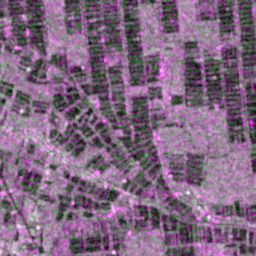
\includegraphics[width=0.2\textwidth, height=0.2\textheight, keepaspectratio]{img/qualitative-20/sample_1/sar.png} &
        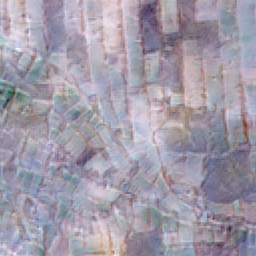
\includegraphics[width=0.2\textwidth, height=0.2\textheight, keepaspectratio]{img/qualitative-20/sample_1/gen.png} &
        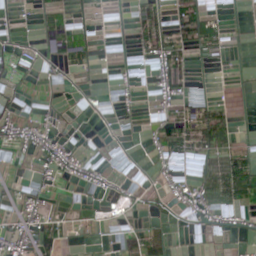
\includegraphics[width=0.2\textwidth, height=0.2\textheight, keepaspectratio]{img/qualitative-20/sample_1/gt.png} \\
        % ------------------- Row 2 -------------------
        \textbf{(b)} &
        \includegraphics[width=0.2\textwidth, height=0.2\textheight, keepaspectratio]{img/qualitative-20/sample_3/sar.png} &
        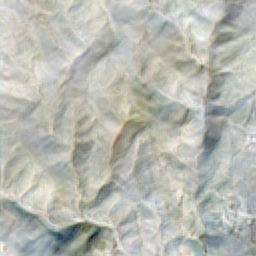
\includegraphics[width=0.2\textwidth, height=0.2\textheight, keepaspectratio]{img/qualitative-20/sample_3/gen.png} &
        \includegraphics[width=0.2\textwidth, height=0.2\textheight, keepaspectratio]{img/qualitative-20/sample_3/gt.png} \\
        \textbf{(c)} &
        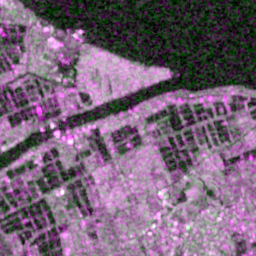
\includegraphics[width=0.2\textwidth, height=0.2\textheight, keepaspectratio]{img/qualitative-20/sample_5/sar.png} &
        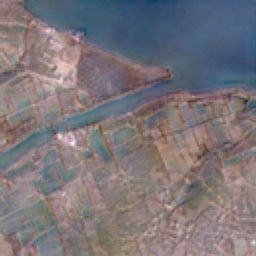
\includegraphics[width=0.2\textwidth, height=0.2\textheight, keepaspectratio]{img/qualitative-20/sample_5/gen.png} &
        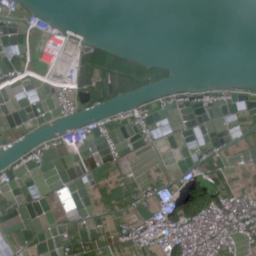
\includegraphics[width=0.2\textwidth, height=0.2\textheight, keepaspectratio]{img/qualitative-20/sample_5/gt.png} \\
        % ------------------- Row 6 -------------------
        \textbf{(d)} &
        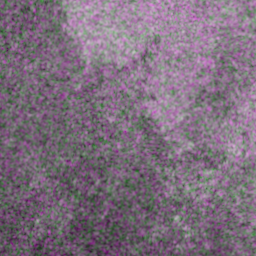
\includegraphics[width=0.2\textwidth, height=0.2\textheight, keepaspectratio]{img/qualitative-20/sample_7/sar.png} &
        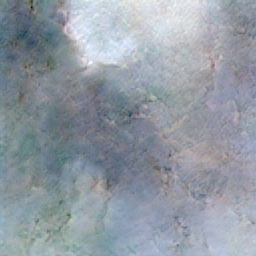
\includegraphics[width=0.2\textwidth, height=0.2\textheight, keepaspectratio]{img/qualitative-20/sample_7/gen.png} &
        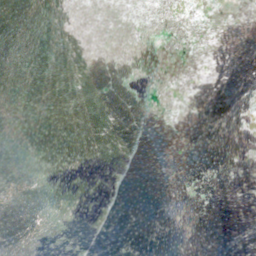
\includegraphics[width=0.2\textwidth, height=0.2\textheight, keepaspectratio]{img/qualitative-20/sample_7/gt.png} \\
    \end{tabular}

    \caption[Qualitative results of 20\% training winter subset]{%
    Qualitative comparison showing representative SAR-to-optical translation results (rows). Columns: 
    \textbf{(i)}~SAR input (pseudo RGB), 
    \textbf{(ii)}~model-generated optical image, 
    \textbf{(iii)}~ground-truth Sentinel-2 image (RGB).
    }
    \label{fig:qualitative_results_20}
\end{figure}

\section{Results on the Full Winter Subset}
GAN-based models generally require large amounts of training data to achieve high-quality image generation, particularly when using mono-temporal SAR imagery as input for translation to optical domains~\cite{sar_2_opt_CGAN_survey_taxonomy}, and especially when reconstructing the full spectral range. Since training on only 20\% of the dataset did not yield satisfactory results, an additional experiment was conducted using the full winter subset, which comprises 31,825 samples divided in an 8:1:1 ratio for training, validation, and testing. This corresponds to approximately 25,460 samples for training and 3,180 samples each for validation and testing. The data preprocessing procedure, training pipeline, and hyperparameters were kept identical to those used in the 20\% experiment to ensure that the effect of training data size was isolated and directly evaluated.

The model required approximately 25$\sim$hours to complete 150~epochs of training. The experimental hypothesis was confirmed: increasing the size of the training dataset led to a clear improvement in model performance. As shown in Table~\ref{tab:quantitative_result_scale}, expanding the training data from 20\% to the full winter subset resulted in substantial gains across all evaluation metrics. In particular, the LPIPS score decreased from 0.224 to 0.173, indicating that the model trained on the full dataset produced outputs with higher perceptual similarity to the ground truth. Likewise, the median SAM value dropped from 6.71° to 4.41°, demonstrating a notable enhancement in spectral consistency across all bands. Furthermore, PSNR increased by approximately 5$\sim$dB, while MAE and RMSE decreased by more than 25\%, confirming the strong positive effect of data scale on reconstruction quality.

\begin{table}[h!]
    \centering
    \caption[Quantitative results for different training data scales: 20\% \& 100\%]{Quantitative results of training on 20\% and 100\% of the winter subset. Arrows ($\uparrow$ / $\downarrow$) indicate whether higher or lower values denote better performance, respectively.}
    \begin{tabular}{lcccccc}
        \toprule
        \textbf{Training Data} & \textbf{SSIM $\uparrow$} & \textbf{PSNR (dB) $\uparrow$} & \textbf{LPIPS $\downarrow$} & \textbf{SAM (°) $\downarrow$} & \textbf{MAE $\downarrow$} & \textbf{RMSE $\downarrow$} \\
        \midrule
        20\% of subset         & 0.859                    & 27.65                         & 0.224                       & 6.71                          & 195.30                    & 381.57                     \\
        100\% of subset        & \textbf{0.888}           & \textbf{32.63}                & \textbf{0.173}              & \textbf{4.41}                 & \textbf{140.72}           & \textbf{233.69}            \\
        \bottomrule
    \end{tabular}
    \label{tab:quantitative_result_scale}
\end{table} 
Similarly, the image reconstruction quality improves noticeably with a larger training dataset. Qualitative examples are shown in Figure~\ref{fig:qualitative_results_100_20}. The model trained on the full winter subset not only better preserves the structural details of the reference images but also achieves markedly enhanced color fidelity, as evident in column (a). In the urban scene (b), it accurately reconstructs the city layout and successfully delineates the river traversing the area. Furthermore, compared to the model trained on only 20\% of the data, the full-data model better captures surface relief and elevation depth, as illustrated in (c).

These qualitative and quantitative improvements demonstrate that increasing the amount and diversity of training data enables the model to more effectively learn both the perceptual and spectral characteristics of the optical domain, ultimately guiding it toward more realistic and color-consistent reconstructions.

\begin{figure}[h!]
    \centering
    \setlength{\tabcolsep}{2pt} % horizontal padding between columns (same as ablation)
    \renewcommand{\arraystretch}{1.0} % vertical padding (same as ablation)

    \begin{tabular}{c *{4}{c}}
        % ------------------- Row 1 -------------------
        \textbf{(a)} &
        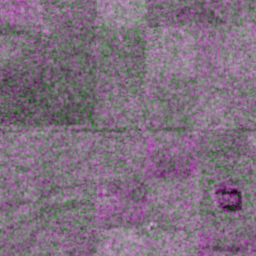
\includegraphics[width=0.2\textwidth, height=0.2\textheight, keepaspectratio]{img/qualitative-20-full/sample_1/sar.png} &
        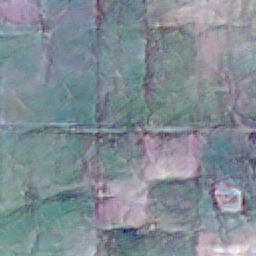
\includegraphics[width=0.2\textwidth, height=0.2\textheight, keepaspectratio]{img/qualitative-20-full/sample_1/gen_0.2.png} &
        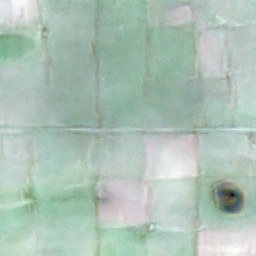
\includegraphics[width=0.2\textwidth, height=0.2\textheight, keepaspectratio]{img/qualitative-20-full/sample_1/gen_full.png} &
        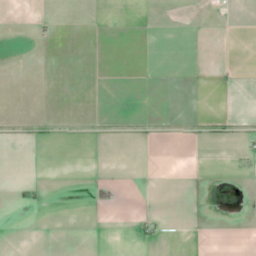
\includegraphics[width=0.2\textwidth, height=0.2\textheight, keepaspectratio]{img/qualitative-20-full/sample_1/gt.png} \\
        % ------------------- Row 2 -------------------
        \textbf{(b)} &
        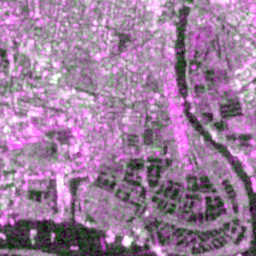
\includegraphics[width=0.2\textwidth, height=0.2\textheight, keepaspectratio]{img/qualitative-20-full/sample_2/sar.png} &
        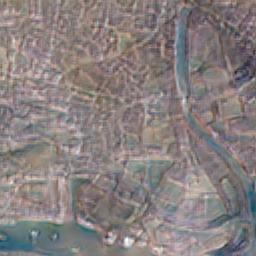
\includegraphics[width=0.2\textwidth, height=0.2\textheight, keepaspectratio]{img/qualitative-20-full/sample_2/gen_0.2.png} &
        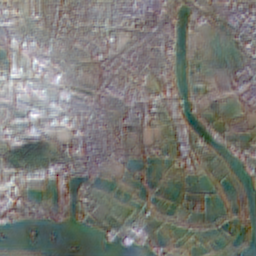
\includegraphics[width=0.2\textwidth, height=0.2\textheight, keepaspectratio]{img/qualitative-20-full/sample_2/gen_full.png} &
        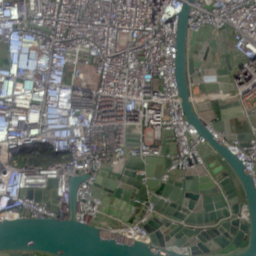
\includegraphics[width=0.2\textwidth, height=0.2\textheight, keepaspectratio]{img/qualitative-20-full/sample_2/gt.png} \\
        \textbf{(c)} &
        \includegraphics[width=0.2\textwidth, height=0.2\textheight, keepaspectratio]{img/qualitative-20-full/sample_3/sar.png} &
        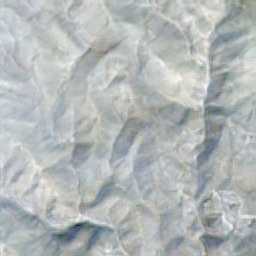
\includegraphics[width=0.2\textwidth, height=0.2\textheight, keepaspectratio]{img/qualitative-20-full/sample_3/gen_0.2.png} &
        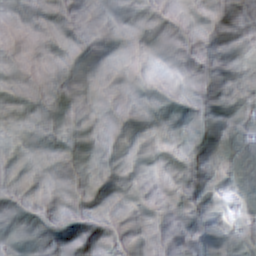
\includegraphics[width=0.2\textwidth, height=0.2\textheight, keepaspectratio]{img/qualitative-20-full/sample_3/gen_full.png} &
        \includegraphics[width=0.2\textwidth, height=0.2\textheight, keepaspectratio]{img/qualitative-20-full/sample_3/gt.png} \\
        % ------------------- Row 6 -------------------
        \textbf{(d)} &
        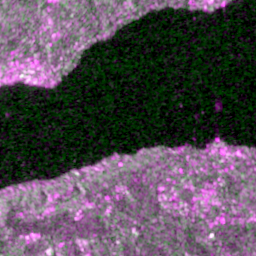
\includegraphics[width=0.2\textwidth, height=0.2\textheight, keepaspectratio]{img/qualitative-20-full/sample_4/sar.png} &
        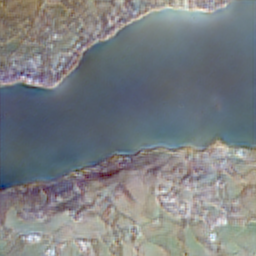
\includegraphics[width=0.2\textwidth, height=0.2\textheight, keepaspectratio]{img/qualitative-20-full/sample_4/gen_0.2.png} &
        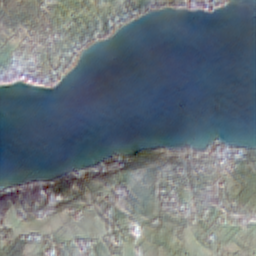
\includegraphics[width=0.2\textwidth, height=0.2\textheight, keepaspectratio]{img/qualitative-20-full/sample_4/gen_full.png} &
        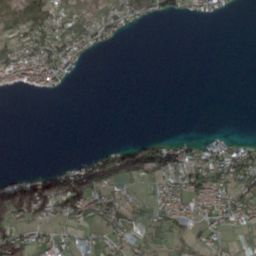
\includegraphics[width=0.2\textwidth, height=0.2\textheight, keepaspectratio]{img/qualitative-20-full/sample_4/gt.png} \\
    \end{tabular}

    \caption[Qualitative results for different training data scales: 20\% \& 100\%]{%
    Qualitative comparison of models trained on 20\% and 100\% of the dataset. 
    Columns: \textbf{(i)}~SAR input (pseudo-RGB), 
    \textbf{(ii)}~generated optical image from 20\% training, 
    \textbf{(iii)}~generated optical image from 100\% training, and 
    \textbf{(iv)}~ground-truth Sentinel-2 image. All optical images are depicted in RGB (B4, B4, B2) batch.}
    \label{fig:qualitative_results_100_20}
\end{figure}

\section{Results Across Individual Optical Bands}
Another objective of this work was to assess the model’s ability to reliably reconstruct each optical band individually and to evaluate the extent of its accuracy across the spectrum. 
For this purpose, the model trained on the full winter subset was evaluated separately for all Sentinel-2 bands, and the corresponding results are summarized in Table~\ref{tab:per_band_validation}.

When comparing the reconstruction quality across individual bands, the focus is placed on the unitless SSIM metric. Other metrics such as MAE or RMSE are not directly comparable between bands, as they depend on the absolute magnitude and statistical distribution of reflectance values, which differ across spectral ranges. In contrast, SSIM measures local structural similarity based on relative intensity patterns rather than absolute values. While not entirely invariant to scale differences, SSIM provides a more robust and interpretable basis for cross-band comparison in this context.

\begin{table}[h!]
\centering
\caption[Per-band validation results for full dataset training]{%
Per-band quantitative validation results of the \textit{pix2pix} model trained on the full winter subset. Each Sentinel-2 band’s central wavelength, spectral designation, and native spatial resolution are listed for reference.}
\resizebox{0.9\textwidth}{!}{%
\begin{tabular}{lcccc}
\toprule
\textbf{Band} & \textbf{PSNR (dB) $\uparrow$} & \textbf{SSIM $\uparrow$} & \textbf{Central Wavelength [nm]} & \textbf{Spectral / Resolution [m]} \\
\midrule
B1   &  36.53  &  0.9758 & 443  & Aerosols / 60 \\
B2   &  37.49  &  0.9506 & 490  & Blue / 10 \\
B3   &  35.67  &  0.9199 & 560  & Green / 10 \\
B4   &  32.84  &  0.8639 & 665  & Red / 10 \\
B5   &  33.68  &  0.9007 & 705  & Red Edge / 20 \\
B6   &  31.62  &  0.8536 & 740  & Red Edge / 20 \\
B7   &  30.37  &  0.8253 & 783  & Red Edge / 20 \\
B8   &  29.62  &  0.7738 & 842  & NIR / 10 \\
B8A  &  29.62  &  0.8071 & 865  & Red Edge / 20 \\
B9   &  33.99  &  0.9388 & 945  & Water Vapour / 60 \\
B10  &  32.12  &  0.9386 & 1375 & Cirrus / 60 \\
B11  &  29.92  &  0.8309 & 1610 & SWIR / 20 \\
B12  &  31.48  &  0.8586 & 2190 & SWIR / 20 \\
\bottomrule
\end{tabular}% 
}
\label{tab:per_band_validation}
\end{table}

Notably, Band~8 (NIR), despite its native spatial resolution of 10~m, exhibits the lowest reconstruction performance among all bands, including those at coarser resolutions, as illustrated in Figure~\ref{fig:ssim_per_band}. This suggests a weaker correlation between SAR backscatter and NIR reflectance compared to other spectral regions, likely due to their differing sensitivity to surface structure and vegetation properties. In contrast, the 60~m atmospheric correction bands—B1 (Aerosols), B9 (Water Vapour), and B10 (Cirrus)—are reconstructed reliably, with B1 achieving the highest SSIM overall. Their smoother spectral characteristics and lower spatial variability likely facilitate more stable and accurate predictions, even after resampling to 10 m.

\begin{figure}[h!]
\centering
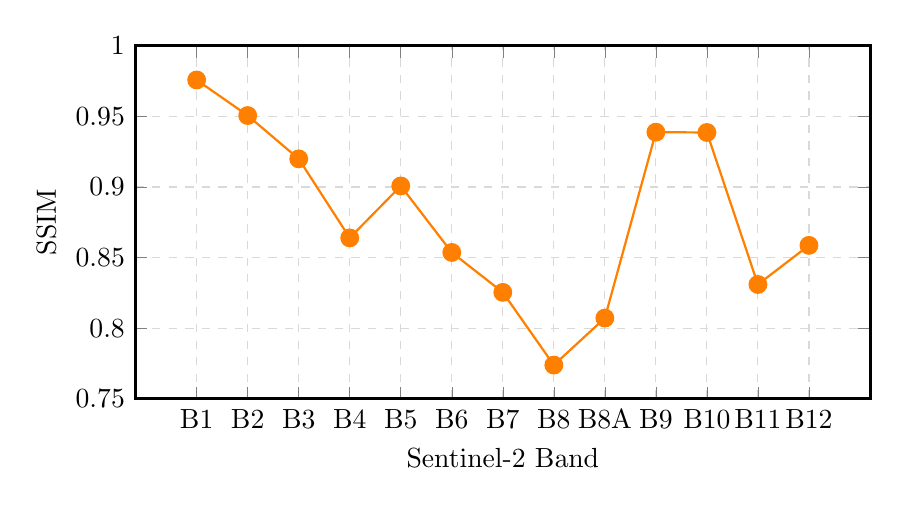
\begin{tikzpicture}
\begin{axis}[
    width=0.9\textwidth,
    height=0.5\textwidth,
    xlabel={Sentinel-2 Band},
    ylabel={SSIM},
    ymin=0.75, ymax=1.0,
    ytick distance=0.05,
    xtick=data,
    xticklabels={B1,B2,B3,B4,B5,B6,B7,B8,B8A,B9,B10,B11,B12},
    grid=major,
    grid style={dashed,gray!30},
    every axis plot/.append style={thick, mark=*},
    mark size=3pt,
    line width=1pt,
]

\addplot[
    color=orange,
    mark=*,
    mark options={fill=orange},
]
coordinates {
    (1,0.9758)
    (2,0.9506)
    (3,0.9199)
    (4,0.8639)
    (5,0.9007)
    (6,0.8536)
    (7,0.8253)
    (8,0.7738)
    (9,0.8071)
    (10,0.9388)
    (11,0.9386)
    (12,0.8309)
    (13,0.8586)
};

\end{axis}
\end{tikzpicture}
\caption[Per-band SSIM for the Pix2Pix model]{Per-band SSIM for the \textit{pix2pix} model trained on the full winter subset.}
\label{fig:ssim_per_band}
\end{figure}

To visually complement the quantitative assessment, representative grayscale examples for each Sentinel-2 band are provided in Appendix~\ref{appendix:bandwise_results}. Each example illustrates the generated band alongside its corresponding ground-truth reference, enabling a direct visual evaluation of the reconstruction quality and spatial consistency across the spectrum.

\newpage

\section{Ablation Studies}
\subsection{Effect of Loss Functions}
\label{subsec:ablation_loss}

To evaluate the contribution of each loss component to the overall model performance, an ablation study was conducted. Four training configurations were compared:
\begin{enumerate}
    \item $\mathcal{L}_{\text{GAN}} + \mathcal{L}_{\text{L1}}$,
    \item $\mathcal{L}_{\text{GAN}} + \mathcal{L}_{\text{L1}} + \mathcal{L}_{\text{SSIM}}$,
    \item $\mathcal{L}_{\text{GAN}} + \mathcal{L}_{\text{L1}} + \mathcal{L}_{\text{LPIPS}}$, and
    \item the full combination $\mathcal{L}_{\text{GAN}} + \mathcal{L}_{\text{L1}} + \mathcal{L}_{\text{SSIM}} + \mathcal{L}_{\text{LPIPS}}$.
\end{enumerate}
This analysis aimed to isolate the contribution of each additional loss term to both quantitative performance and visual reconstruction quality. The evaluation was conducted using the same IQA metrics employed throughout the thesis, namely SSIM, PSNR, LPIPS, SAM, MAE, and RMSE. Several training loops were conducted using the same preprocessing procedure described in Section~\ref{subsec:preprocessing}. All models were trained under identical settings, hyperparameters, datasets, and number of epochs to ensure a fair and consistent comparison across the different loss configurations.

Table~\ref{tab:ablation_quantitative} summarizes the quantitative performance across the four loss configurations. As shown, the baseline configuration without SSIM and LPIPS achieved the lowest performance across most metrics, with the exception of PSNR. This configuration also represents the weakest setup in terms of overall image quality. As illustrated in Figure~\ref{fig:ablation_samples}(b), images generated by the baseline model differ significantly from the ground truth, both texturally and perceptually. 

\begin{table}[h!]
    \centering
    \resizebox{\textwidth}{!}{%
        \begin{tabular}{lcccccc}
            \toprule
            \textbf{Loss Configuration}                                                                                   & \textbf{SSIM $\uparrow$} & \textbf{PSNR (dB) $\uparrow$} & \textbf{LPIPS $\downarrow$} & \textbf{SAM~(°) $\downarrow$} & \textbf{MAE $\downarrow$} & \textbf{RMSE $\downarrow$} \\
            \midrule
            $\mathcal{L}_{\text{GAN}} + \mathcal{L}_{\text{L1}}$                                                          & 0.820                    & 26.38                         & 0.287                       & 6.47                          & 229                       & 441                        \\
            $\mathcal{L}_{\text{GAN}} + \mathcal{L}_{\text{L1}} + \mathcal{L}_{\text{SSIM}}$                              & \textbf{0.862}           & \textbf{27.67}                & 0.399                       & \textbf{5.43}                 & 198                       & \textbf{380}               \\
            $\mathcal{L}_{\text{GAN}} + \mathcal{L}_{\text{L1}} + \mathcal{L}_{\text{LPIPS}}$                             & 0.842                    & 27.58                         & \textbf{0.213}              & 5.73                          & 201                       & 385                        \\
            $\mathcal{L}_{\text{GAN}} + \mathcal{L}_{\text{L1}} + \mathcal{L}_{\text{SSIM}} + \mathcal{L}_{\text{LPIPS}}$ & 0.859                    & 27.65                         & 0.224                       & 5.44                          & \textbf{195}              & 382                        \\
            \bottomrule
        \end{tabular}%
    }
    \caption[Quantitative ablation study across loss configurations]{Quantitative results of the ablation study across different loss configurations. Best values per metric are shown in bold.}
    \label{tab:ablation_quantitative}
\end{table}

Notably, integrating SSIM alone yielded the highest quantitative scores in several metrics. However, the qualitative results under this configuration reveal perceptual inconsistencies and reduced visual realism. This discrepancy arises because SSIM does not always align with human perceptual judgments of image similarity. As reported by NVIDIA in~\cite{nvidia_Understanding_SSIM}, SSIM can overemphasize small intensity variations in dark regions, overlook significant color shifts, and assign high similarity near edges even when visible artifacts are present.

\begin{figure}[h!]
    \centering
    \setlength{\tabcolsep}{2pt} % horizontal padding between columns
    \renewcommand{\arraystretch}{1.0} % vertical padding

    % Adjust width so that 6 images fit one row across the text width
    % (tweak 0.155\textwidth to 0.158 or 0.152 if needed)
    \begin{tabular}{*{6}{c}}
        % \toprule
        (a) & (b) & (c) & (d) & (e) & (f) \\
        % \midrule

        % ------------------- Row 1 -------------------
        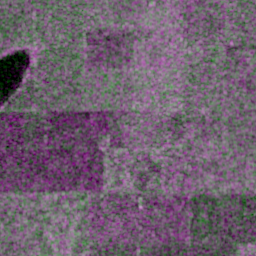
\includegraphics[width=0.155\textwidth]{img/ablation/sample_1/sar.png}   &
        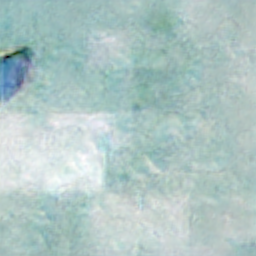
\includegraphics[width=0.155\textwidth]{img/ablation/sample_1/none.png}  &
        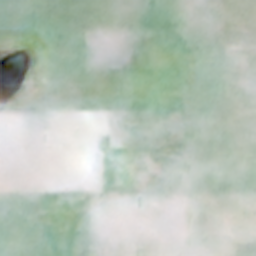
\includegraphics[width=0.155\textwidth]{img/ablation/sample_1/ssim.png}  &
        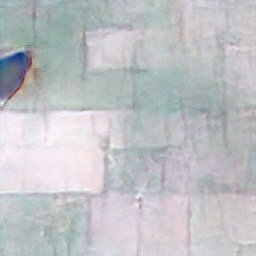
\includegraphics[width=0.155\textwidth]{img/ablation/sample_1/lpips.png} &
        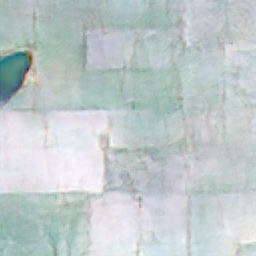
\includegraphics[width=0.155\textwidth]{img/ablation/sample_1/all.png}   &
        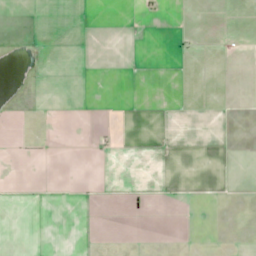
\includegraphics[width=0.155\textwidth]{img/ablation/sample_1/gt.png}                                  \\
        % ------------------- Row 2 -------------------
        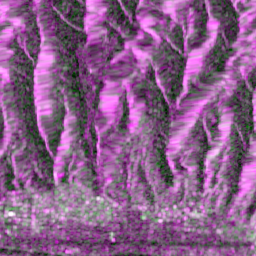
\includegraphics[width=0.155\textwidth]{img/ablation/sample_2/sar.png}   &
        \includegraphics[width=0.155\textwidth]{img/ablation/sample_2/none.png}  &
        \includegraphics[width=0.155\textwidth]{img/ablation/sample_2/ssim.png}  &
        \includegraphics[width=0.155\textwidth]{img/ablation/sample_2/lpips.png} &
        \includegraphics[width=0.155\textwidth]{img/ablation/sample_2/all.png}   &
        \includegraphics[width=0.155\textwidth]{img/ablation/sample_2/gt.png}                                  \\
        % ------------------- Row 3 -------------------
        \includegraphics[width=0.155\textwidth]{img/ablation/sample_3/sar.png}   &
        \includegraphics[width=0.155\textwidth]{img/ablation/sample_3/none.png}  &
        \includegraphics[width=0.155\textwidth]{img/ablation/sample_3/ssim.png}  &
        \includegraphics[width=0.155\textwidth]{img/ablation/sample_3/lpips.png} &
        \includegraphics[width=0.155\textwidth]{img/ablation/sample_3/all.png}   &
        \includegraphics[width=0.155\textwidth]{img/ablation/sample_3/gt.png}                                  \\
        % ------------------- Row 4 -------------------
        \includegraphics[width=0.155\textwidth]{img/ablation/sample_4/sar.png}   &
        \includegraphics[width=0.155\textwidth]{img/ablation/sample_4/none.png}  &
        \includegraphics[width=0.155\textwidth]{img/ablation/sample_4/ssim.png}  &
        \includegraphics[width=0.155\textwidth]{img/ablation/sample_4/lpips.png} &
        \includegraphics[width=0.155\textwidth]{img/ablation/sample_4/all.png}   &
        \includegraphics[width=0.155\textwidth]{img/ablation/sample_4/gt.png}                                  \\
        % \bottomrule
    \end{tabular}

    \caption[Qualitative ablation study across loss configurations]{%
    Qualitative ablation results showing representative samples (rows) under four configurations (columns):\\
    \textbf{(a)}~Input SAR (pseudo RGB)\\
    \textbf{(b)}~$\mathcal{L}_{\text{GAN}}{+}\mathcal{L}_{\text{L1}}$\\
    \textbf{(c)}~$\mathcal{L}_{\text{GAN}}{+}\mathcal{L}_{\text{L1}}{+}\mathcal{L}_{\text{SSIM}}$\\
    \textbf{(d)}~$\mathcal{L}_{\text{GAN}}{+}\mathcal{L}_{\text{L1}}{+}\mathcal{L}_{\text{LPIPS}}$\\
    \textbf{(e)}~all four losses combined\\
    \textbf{(f)}~ground-truth Sentinel-2 optical image (RGB bands).
    }
    \label{fig:ablation_samples}
\end{figure}

Since the primary objective of LPIPS is to measure perceptual similarity, incorporating it into the baseline configuration led to notable improvements in the preservation of low-level features. As illustrated in column~(d) of Figure~\ref{fig:ablation_samples}, the model was able to maintain sharper edges and more distinct boundaries. Moreover, the generated images appear visually more realistic and closely resemble the ground truth in texture and detail. However, the colour reproduction achieved with LPIPS is slightly inferior to that obtained using SSIM, as the SSIM-based model produces more natural and accurate colours overall.

The full combination of all four losses achieved the best balance between pixel-level accuracy, perceptual realism, and structural coherence. 
Its SAM values were the second best, differing only marginally from the SSIM-only configuration. 
By incorporating both SSIM and LPIPS, the model attains an effective balance between color, luminance, and perceptual realism, as shown in column~(e) of Figure~\ref{fig:ablation_samples}. 
Similar findings were also reported by~\cite{s2o_ViT_cGAN} and~\cite{CR_RS_GAN_s2o}. 
 
Overall, the results demonstrate the incremental benefit of incorporating perceptual and structural similarity terms alongside the adversarial $\mathcal{L}_{\text{GAN}}$ and $\mathrm{L1}$ objectives. 

\subsection{Effect of Excluding 60 m Bands}
Given the varying data distributions and the originally different spatial resolutions of the Sentinel-2 bands (even though all were resampled to 10m in the dataset), it was hypothesized that including the 60m bands might introduce noise and confuse the model during training. To examine this assumption, an ablation study was conducted using the same training configuration as for the full 13-band model, both trained on 20\% of the winter subset.

Surprisingly, removing the 60m bands did not lead to any improvement. Instead, both SSIM and LPIPS scores decreased, as reported in Table~\ref{tab:ablation_excluding_60m}. This suggests that the 60m bands, which primarily serve for atmospheric correction (e.g., B1, B9, and B10), provide complementary spectral information that contributes to maintaining spectral fidelity during training.

\begin{table}[h!]
    \centering
    \setlength{\tabcolsep}{8pt}
    \renewcommand{\arraystretch}{1.15}
    \caption[[Overall performance when excluding 60m bands]]{Overall performance comparing all 13 bands vs. excluding the 60m bands (B1, B9, B10).}
    \label{tab:ablation_excluding_60m}
    \begin{tabular}{lccc}
        \hline
        \textbf{Setting} & \textbf{SSIM $\uparrow$} & \textbf{PSNR (dB) $\uparrow$} & \textbf{SAM~(°) $\downarrow$} \\
        \hline
        All 13 bands & 0.859390 & 27.650251 & 6.7064 \\
        Excluding 60m (B1,B9,B10) & 0.825861 & 26.474423 & 6.3339 \\
        \hline
    \end{tabular}
    % Note: SAM is computed in 13-band space for "All 13 bands" and in 10-band space when excluding 60 m bands.
\end{table}

Interestingly, while the SAM slightly improved after excluding the 60m bands, this does not necessarily contradict the decline in PSNR and SSIM. The model may have learned to reproduce more spectrally consistent relationships between the remaining bands (hence a smaller spectral angle), yet failed to preserve the absolute reflectance magnitudes and spatial details, leading to lower overall reconstruction quality. This indicates a trade-off between radiometric fidelity and spectral coherence in the absence of the full spectral range. For qualitative evaluation, Figure~\ref{fig:ablation_excluding_60m_qualitative} illustrates the generated optical images obtained from models trained with the full spectral configuration and with the 60,m bands excluded.

Similarly, the per-band evaluation (Table~\ref{tab:ablation_excluding_60m_per_band}) confirms this trend. For most bands, SSIM remains stable when all bands are included, indicating consistent structural reconstruction quality. However, PSNR decreases for nearly all bands when the 60m bands are excluded, with the exception of B1, demonstrating that the full spectral configuration better supports radiometric reconstruction.
\begin{figure}[h!]
    \centering
    \setlength{\tabcolsep}{2pt} % horizontal padding between columns
    \renewcommand{\arraystretch}{1.0} % vertical padding

    \begin{tabular}{cccc}
        % ------------------- Rows -------------------
        \includegraphics[width=0.2\textwidth, height=0.2\textheight, keepaspectratio]{img/exclusion_60_m/bands10/sample_000034_sar_pseudo.png} &
        \includegraphics[width=0.2\textwidth, height=0.2\textheight, keepaspectratio]{img/exclusion_60_m/bands10/sample_000034_pred_rgb.png} &
        \includegraphics[width=0.2\textwidth, height=0.2\textheight, keepaspectratio]{img/exclusion_60_m/bands13/sample_000034_pred_rgb.png} &
        \includegraphics[width=0.2\textwidth, height=0.2\textheight, keepaspectratio]{img/exclusion_60_m/bands10/sample_000034_true_rgb.png} \\

        \includegraphics[width=0.2\textwidth, height=0.2\textheight, keepaspectratio]{img/exclusion_60_m/bands10/sample_000050_sar_pseudo.png} &
        \includegraphics[width=0.2\textwidth, height=0.2\textheight, keepaspectratio]{img/exclusion_60_m/bands10/sample_000050_pred_rgb.png} &
        \includegraphics[width=0.2\textwidth, height=0.2\textheight, keepaspectratio]{img/exclusion_60_m/bands13/sample_000050_pred_rgb.png} &
        \includegraphics[width=0.2\textwidth, height=0.2\textheight, keepaspectratio]{img/exclusion_60_m/bands10/sample_000050_true_rgb.png} \\

        \includegraphics[width=0.2\textwidth, height=0.2\textheight, keepaspectratio]{img/exclusion_60_m/bands10/sample_000010_sar_pseudo.png} &
        \includegraphics[width=0.2\textwidth, height=0.2\textheight, keepaspectratio]{img/exclusion_60_m/bands10/sample_000010_pred_rgb.png} &
        \includegraphics[width=0.2\textwidth, height=0.2\textheight, keepaspectratio]{img/exclusion_60_m/bands13/sample_000010_pred_rgb.png} &
        \includegraphics[width=0.2\textwidth, height=0.2\textheight, keepaspectratio]{img/exclusion_60_m/bands10/sample_000010_true_rgb.png} \\

        \includegraphics[width=0.2\textwidth, height=0.2\textheight, keepaspectratio]{img/exclusion_60_m/bands10/sample_000065_sar_pseudo.png} &
        \includegraphics[width=0.2\textwidth, height=0.2\textheight, keepaspectratio]{img/exclusion_60_m/bands10/sample_000065_pred_rgb.png} &
        \includegraphics[width=0.2\textwidth, height=0.2\textheight, keepaspectratio]{img/exclusion_60_m/bands13/sample_000065_pred_rgb.png} &
        \includegraphics[width=0.2\textwidth, height=0.2\textheight, keepaspectratio]{img/exclusion_60_m/bands10/sample_000065_true_rgb.png} \\
    \end{tabular}

    \caption[Qualitative results when excluding 60\,m bands]{%
    Qualitative comparison of generated optical images when excluding the 60\,m Sentinel-2 bands. 
    Columns: \textbf{(i)}~SAR input (pseudo-RGB), 
    \textbf{(ii)}~generated optical image trained without the 60\,m bands, 
    \textbf{(iii)}~generated optical image trained with all 13 bands, and 
    \textbf{(iv)}~reference cloud-free Sentinel-2 image. 
    All optical outputs are visualized in RGB composition (B4, B3, B2).}
    \label{fig:ablation_excluding_60m_qualitative}
\end{figure}

\begin{table}[h!]
    \centering
    \setlength{\tabcolsep}{6pt}
    \renewcommand{\arraystretch}{1.15}
    \caption[Per-band performance when excluding 60m bands]{Per-band comparison of SSIM and PSNR. Columns are ordered as SSIM (no 60\,m), SSIM (13), PSNR (no 60\,m), and PSNR (13). A dash indicates the band was excluded in the 60\,m-removed setting.}
    \label{tab:ablation_excluding_60m_per_band}
    \begin{tabular}{lcccc}
        \hline
        Band & SSIM (no 60\,m) $\uparrow$ & SSIM (13) $\uparrow$ & PSNR (no 60\,m) [dB] $\uparrow$ & PSNR (13) [dB] $\uparrow$ \\
        \hline
        B1   & ---    & 0.9634 & ---    & 29.749 \\
        B2   & 0.9431 & 0.9430 & 34.151 & 34.057 \\
        B3   & 0.9064 & 0.9060 & 31.691 & 31.718 \\
        B4   & 0.8348 & 0.8340 & 28.039 & 28.145 \\
        B5   & 0.8707 & 0.8729 & 28.098 & 28.257 \\
        B6   & 0.8199 & 0.8231 & 26.740 & 26.926 \\
        B7   & 0.7890 & 0.7925 & 25.694 & 25.884 \\
        B8   & 0.7375 & 0.7416 & 25.534 & 25.739 \\
        B8A  & 0.7687 & 0.7722 & 25.095 & 25.311 \\
        B9   & ---    & 0.8666 & ---    & 24.617 \\
        B10  & ---    & 0.8826 & ---    & 24.571 \\
        B11  & 0.7774 & 0.7809 & 23.395 & 23.727 \\
        B12  & 0.8034 & 0.8073 & 24.956 & 25.263 \\
        \hline
    \end{tabular}
\end{table}


\chapter{Ablation Studies}
\section{Effect of Loss Functions}
\label{subsec:ablation_loss}

To evaluate the contribution of each loss component to the overall model performance, an ablation study was conducted. Four training configurations were compared:
\begin{enumerate}
    \item $\mathcal{L}_{\text{GAN}} + \mathcal{L}_{\text{L1}}$,
    \item $\mathcal{L}_{\text{GAN}} + \mathcal{L}_{\text{L1}} + \mathcal{L}_{\text{SSIM}}$,
    \item $\mathcal{L}_{\text{GAN}} + \mathcal{L}_{\text{L1}} + \mathcal{L}_{\text{LPIPS}}$, and
    \item the full combination $\mathcal{L}_{\text{GAN}} + \mathcal{L}_{\text{L1}} + \mathcal{L}_{\text{SSIM}} + \mathcal{L}_{\text{LPIPS}}$.
\end{enumerate}
This analysis aimed to isolate the contribution of each additional loss term to both quantitative performance and visual reconstruction quality. The evaluation was conducted using the same IQA metrics employed throughout the thesis, namely SSIM, PSNR, LPIPS, SAM, MAE, and RMSE. Several training loops were conducted using the same preprocessing procedure described in Section~\ref{subsec:preprocessing}. All models were trained under identical settings, hyperparameters, datasets, and number of epochs to ensure a fair and consistent comparison across the different loss configurations.

Table~\ref{tab:ablation_quantitative} summarizes the quantitative performance across the four loss configurations. As shown, the baseline configuration without SSIM and LPIPS achieved the lowest performance across most metrics, with the exception of PSNR. This configuration also represents the weakest setup in terms of overall image quality. As illustrated in Figure~\ref{fig:ablation_samples}(b), images generated by the baseline model differ significantly from the ground truth, both texturally and perceptually. 

\begin{table}[h!]
    \centering
    \resizebox{\textwidth}{!}{%
        \begin{tabular}{lcccccc}
            \toprule
            \textbf{Loss Configuration}                                                                                   & \textbf{SSIM $\uparrow$} & \textbf{PSNR (dB) $\uparrow$} & \textbf{LPIPS $\downarrow$} & \textbf{SAM~(°) $\downarrow$} & \textbf{MAE $\downarrow$} & \textbf{RMSE $\downarrow$} \\
            \midrule
            $\mathcal{L}_{\text{GAN}} + \mathcal{L}_{\text{L1}}$                                                          & 0.820                    & 26.38                         & 0.287                       & 7.88                          & 229                       & 441                        \\
            $\mathcal{L}_{\text{GAN}} + \mathcal{L}_{\text{L1}} + \mathcal{L}_{\text{SSIM}}$                              & \textbf{0.862}           & \textbf{27.67}                & 0.399                       & \textbf{6.67}                 & 198                       & \textbf{380}               \\
            $\mathcal{L}_{\text{GAN}} + \mathcal{L}_{\text{L1}} + \mathcal{L}_{\text{LPIPS}}$                             & 0.842                    & 27.58                         & \textbf{0.213}              & 7.05                         & 201                       & 385                        \\
            $\mathcal{L}_{\text{GAN}} + \mathcal{L}_{\text{L1}} + \mathcal{L}_{\text{SSIM}} + \mathcal{L}_{\text{LPIPS}}$ & 0.859                    & 27.65                         & 0.224                       &  6.71                          & \textbf{195}              & 382                        \\
            \bottomrule
        \end{tabular}%
    }
    \caption[Quantitative ablation study across loss configurations]{Quantitative results of the ablation study across different loss configurations. Best values per metric are shown in bold.}
    \label{tab:ablation_quantitative}
\end{table}

Notably, integrating SSIM alone yielded the highest quantitative scores in several metrics. However, the qualitative results under this configuration reveal perceptual inconsistencies and reduced visual realism. This discrepancy arises because SSIM does not always align with human perceptual judgments of image similarity. As reported by NVIDIA in~\cite{nvidia_Understanding_SSIM}, SSIM can overemphasize small intensity variations in dark regions, overlook significant color shifts, and assign high similarity near edges even when visible artifacts are present.

\begin{figure}[h!]
    \centering
    \setlength{\tabcolsep}{2pt} % horizontal padding between columns
    \renewcommand{\arraystretch}{1.0} % vertical padding

    % Adjust width so that 6 images fit one row across the text width
    % (tweak 0.155\textwidth to 0.158 or 0.152 if needed)
    \begin{tabular}{*{6}{c}}
        % \toprule
        (a) & (b) & (c) & (d) & (e) & (f) \\
        % \midrule

        % ------------------- Row 1 -------------------
        \includegraphics[width=0.155\textwidth]{img/ablation/sample_1/sar.png}   &
        \includegraphics[width=0.155\textwidth]{img/ablation/sample_1/none.png}  &
        \includegraphics[width=0.155\textwidth]{img/ablation/sample_1/ssim.png}  &
        \includegraphics[width=0.155\textwidth]{img/ablation/sample_1/lpips.png} &
        \includegraphics[width=0.155\textwidth]{img/ablation/sample_1/all.png}   &
        \includegraphics[width=0.155\textwidth]{img/ablation/sample_1/gt.png}                                  \\
        % ------------------- Row 2 -------------------
        \includegraphics[width=0.155\textwidth]{img/ablation/sample_2/sar.png}   &
        \includegraphics[width=0.155\textwidth]{img/ablation/sample_2/none.png}  &
        \includegraphics[width=0.155\textwidth]{img/ablation/sample_2/ssim.png}  &
        \includegraphics[width=0.155\textwidth]{img/ablation/sample_2/lpips.png} &
        \includegraphics[width=0.155\textwidth]{img/ablation/sample_2/all.png}   &
        \includegraphics[width=0.155\textwidth]{img/ablation/sample_2/gt.png}                                  \\
        % ------------------- Row 3 -------------------
        \includegraphics[width=0.155\textwidth]{img/ablation/sample_3/sar.png}   &
        \includegraphics[width=0.155\textwidth]{img/ablation/sample_3/none.png}  &
        \includegraphics[width=0.155\textwidth]{img/ablation/sample_3/ssim.png}  &
        \includegraphics[width=0.155\textwidth]{img/ablation/sample_3/lpips.png} &
        \includegraphics[width=0.155\textwidth]{img/ablation/sample_3/all.png}   &
        \includegraphics[width=0.155\textwidth]{img/ablation/sample_3/gt.png}                                  \\
        % ------------------- Row 4 -------------------
        \includegraphics[width=0.155\textwidth]{img/ablation/sample_4/sar.png}   &
        \includegraphics[width=0.155\textwidth]{img/ablation/sample_4/none.png}  &
        \includegraphics[width=0.155\textwidth]{img/ablation/sample_4/ssim.png}  &
        \includegraphics[width=0.155\textwidth]{img/ablation/sample_4/lpips.png} &
        \includegraphics[width=0.155\textwidth]{img/ablation/sample_4/all.png}   &
        \includegraphics[width=0.155\textwidth]{img/ablation/sample_4/gt.png}                                  \\
        % \bottomrule
    \end{tabular}

    \caption[Qualitative ablation study across loss configurations]{%
    Qualitative ablation results showing representative samples (rows) under four configurations (columns):\\
    \textbf{(a)}~Input SAR (pseudo RGB)\\
    \textbf{(b)}~$\mathcal{L}_{\text{GAN}}{+}\mathcal{L}_{\text{L1}}$\\
    \textbf{(c)}~$\mathcal{L}_{\text{GAN}}{+}\mathcal{L}_{\text{L1}}{+}\mathcal{L}_{\text{SSIM}}$\\
    \textbf{(d)}~$\mathcal{L}_{\text{GAN}}{+}\mathcal{L}_{\text{L1}}{+}\mathcal{L}_{\text{LPIPS}}$\\
    \textbf{(e)}~all four losses combined\\
    \textbf{(f)}~ground-truth Sentinel-2 optical image (RGB bands).
    }
    \label{fig:ablation_samples}
\end{figure}

Since the primary objective of LPIPS is to measure perceptual similarity, incorporating it into the baseline configuration led to notable improvements in the preservation of low-level features. As illustrated in column~(d) of Figure~\ref{fig:ablation_samples}, the model was able to maintain sharper edges and more distinct boundaries. Moreover, the generated images appear visually more realistic and closely resemble the ground truth in texture and detail. However, the colour reproduction achieved with LPIPS is slightly inferior to that obtained using SSIM, as the SSIM-based model produces more natural and accurate colours overall.

The full combination of all four losses achieved the best balance between pixel-level accuracy, perceptual realism, and structural coherence. 
Its SAM values were the second best, differing only marginally from the SSIM-only configuration. 
By incorporating both SSIM and LPIPS, the model attains an effective balance between color, luminance, and perceptual realism, as shown in column~(e) of Figure~\ref{fig:ablation_samples}. 
Similar findings were also reported by~\cite{s2o_ViT_cGAN} and~\cite{CR_RS_GAN_s2o}. 
 
Overall, the results demonstrate the incremental benefit of incorporating perceptual and structural similarity terms alongside the adversarial $\mathcal{L}_{\text{GAN}}$ and $\mathrm{L1}$ objectives. 

\section{Effect of Excluding 60 m Bands}
Given the varying data distributions and the originally different spatial resolutions of the Sentinel-2 bands (even though all were resampled to 10m in the dataset), it was hypothesized that including the 60m bands might introduce noise and confuse the model during training. To examine this assumption, an ablation study was conducted using the same training configuration as for the full 13-band model, both trained on 20\% of the winter subset.

Surprisingly, removing the 60m bands did not lead to any improvement. Instead, both SSIM and LPIPS scores decreased, as reported in Table~\ref{tab:ablation_excluding_60m}. This suggests that the 60m bands, which primarily serve for atmospheric correction (e.g., B1, B9, and B10), provide complementary spectral information that contributes to maintaining spectral fidelity during training.

\begin{table}[h!]
    \centering
    \setlength{\tabcolsep}{8pt}
    \renewcommand{\arraystretch}{1.15}
    \caption[Overall performance when excluding 60m bands]{Overall performance comparing all 13 bands vs. excluding the 60m bands (B1, B9, B10).}
    \label{tab:ablation_excluding_60m}
    \begin{tabular}{lccc}
        \hline
        \textbf{Setting} & \textbf{SSIM $\uparrow$} & \textbf{PSNR (dB) $\uparrow$} & \textbf{SAM~(°) $\downarrow$} \\
        \hline
        All 13 bands & \textbf{0.859390} & \textbf{27.650251} & 6.7064 \\
        Excluding 60m (B1, B9, B10) & 0.825861 & 26.474423 & \textbf{6.3339} \\
        \hline
    \end{tabular}
    % Note: SAM is computed in 13-band space for "All 13 bands" and in 10-band space when excluding 60 m bands.
\end{table}

Interestingly, while the SAM slightly improved after excluding the 60m bands, this does not necessarily contradict the decline in PSNR and SSIM. The model may have learned to reproduce more spectrally consistent relationships between the remaining bands (hence a smaller spectral angle), yet failed to preserve the absolute reflectance magnitudes and spatial details, leading to lower overall reconstruction quality. This indicates a trade-off between radiometric fidelity and spectral coherence in the absence of the full spectral range. For qualitative evaluation, Figure~\ref{fig:ablation_excluding_60m_qualitative} illustrates the generated optical images obtained from models trained with the full spectral configuration and with the 60,m bands excluded.

Similarly, the per-band evaluation (Table~\ref{tab:ablation_excluding_60m_per_band}) confirms this trend. For most bands, SSIM remains stable when all bands are included, indicating consistent structural reconstruction quality. However, PSNR decreases for nearly all bands when the 60m bands are excluded, with the exception of B1, demonstrating that the full spectral configuration better supports radiometric reconstruction.
\begin{figure}[h!]
    \centering
    \setlength{\tabcolsep}{2pt} % horizontal padding between columns
    \renewcommand{\arraystretch}{1.0} % vertical padding

    \begin{tabular}{cccc}
        % ------------------- Rows -------------------
        (a) & (b) & (c) & (d) \\
        \includegraphics[width=0.2\textwidth, height=0.2\textheight, keepaspectratio]{img/exclusion_60_m/bands10/sample_000034_sar_pseudo.png} &
        \includegraphics[width=0.2\textwidth, height=0.2\textheight, keepaspectratio]{img/exclusion_60_m/bands10/sample_000034_pred_rgb.png} &
        \includegraphics[width=0.2\textwidth, height=0.2\textheight, keepaspectratio]{img/exclusion_60_m/bands13/sample_000034_pred_rgb.png} &
        \includegraphics[width=0.2\textwidth, height=0.2\textheight, keepaspectratio]{img/exclusion_60_m/bands10/sample_000034_true_rgb.png} \\

        \includegraphics[width=0.2\textwidth, height=0.2\textheight, keepaspectratio]{img/exclusion_60_m/bands10/sample_000050_sar_pseudo.png} &
        \includegraphics[width=0.2\textwidth, height=0.2\textheight, keepaspectratio]{img/exclusion_60_m/bands10/sample_000050_pred_rgb.png} &
        \includegraphics[width=0.2\textwidth, height=0.2\textheight, keepaspectratio]{img/exclusion_60_m/bands13/sample_000050_pred_rgb.png} &
        \includegraphics[width=0.2\textwidth, height=0.2\textheight, keepaspectratio]{img/exclusion_60_m/bands10/sample_000050_true_rgb.png} \\

        \includegraphics[width=0.2\textwidth, height=0.2\textheight, keepaspectratio]{img/exclusion_60_m/bands10/sample_000010_sar_pseudo.png} &
        \includegraphics[width=0.2\textwidth, height=0.2\textheight, keepaspectratio]{img/exclusion_60_m/bands10/sample_000010_pred_rgb.png} &
        \includegraphics[width=0.2\textwidth, height=0.2\textheight, keepaspectratio]{img/exclusion_60_m/bands13/sample_000010_pred_rgb.png} &
        \includegraphics[width=0.2\textwidth, height=0.2\textheight, keepaspectratio]{img/exclusion_60_m/bands10/sample_000010_true_rgb.png} \\

        \includegraphics[width=0.2\textwidth, height=0.2\textheight, keepaspectratio]{img/exclusion_60_m/bands10/sample_000065_sar_pseudo.png} &
        \includegraphics[width=0.2\textwidth, height=0.2\textheight, keepaspectratio]{img/exclusion_60_m/bands10/sample_000065_pred_rgb.png} &
        \includegraphics[width=0.2\textwidth, height=0.2\textheight, keepaspectratio]{img/exclusion_60_m/bands13/sample_000065_pred_rgb.png} &
        \includegraphics[width=0.2\textwidth, height=0.2\textheight, keepaspectratio]{img/exclusion_60_m/bands10/sample_000065_true_rgb.png} \\
    \end{tabular}

    \caption[Qualitative results when excluding 60\,m bands]{%
    Qualitative comparison of generated optical images when excluding the 60\,m Sentinel-2 bands. 
    Columns: \textbf{(a)}~SAR input (pseudo-RGB), 
    \textbf{(b)}~generated optical image trained without the 60\,m bands, 
    \textbf{(c)}~generated optical image trained with all 13 bands, and 
    \textbf{(d)}~reference cloud-free Sentinel-2 image.}
    \label{fig:ablation_excluding_60m_qualitative}
\end{figure}

\begin{table}[h!]
    \centering
    \setlength{\tabcolsep}{6pt}
    \renewcommand{\arraystretch}{1.15}
    \caption[Per-band performance when excluding 60m bands]{Per-band performance when excluding 60m bands.}
    \label{tab:ablation_excluding_60m_per_band}
    \begin{tabular}{lcccc}
    \hline
    \textbf{Band} & \textbf{SSIM (no 60\,m)} $\uparrow$ & \textbf{SSIM (13)} $\uparrow$ & \textbf{PSNR (no 60\,m) [dB]} $\uparrow$ & \textbf{PSNR (13) [dB]} $\uparrow$ \\
    \hline
    B1   & ---    & 0.9634 & ---    & 29.749 \\
    B2   & 0.9431 & 0.9430 & 34.151 & 34.057 \\
    B3   & 0.9064 & 0.9060 & 31.691 & 31.718 \\
    B4   & 0.8348 & 0.8340 & 28.039 & 28.145 \\
    B5   & 0.8707 & 0.8729 & 28.098 & 28.257 \\
    B6   & 0.8199 & 0.8231 & 26.740 & 26.926 \\
    B7   & 0.7890 & 0.7925 & 25.694 & 25.884 \\
    B8   & 0.7375 & 0.7416 & 25.534 & 25.739 \\
    B8A  & 0.7687 & 0.7722 & 25.095 & 25.311 \\
    B9   & ---    & 0.8666 & ---    & 24.617 \\
    B10  & ---    & 0.8826 & ---    & 24.571 \\
    B11  & 0.7774 & 0.7809 & 23.395 & 23.727 \\
    B12  & 0.8034 & 0.8073 & 24.956 & 25.263 \\
    \hline
    \end{tabular}
\end{table}


% \begin{table}[h!]
% \centering
% \caption[Quantitative results across data scales and seasonal subsets]{%
% Quantitative performance of the \textit{pix2pix} model across different training data scales and seasonal subsets of the SEN12-MS dataset. Arrows ($\uparrow$ / $\downarrow$) indicate whether higher or lower values denote better performance, respectively.}
% \begin{tabular}{lcccc}
% \toprule
% \textbf{Dataset} & \textbf{SSIM $\uparrow$} & \textbf{PSNR (dB) $\uparrow$} & \textbf{LPIPS $\downarrow$} & \textbf{SAM (°) $\downarrow$} \\
% \midrule
% Winter & \textbf{0.888} & \textbf{32.63} & \textbf{0.173} & \textbf{4.41} \\
% Spring & 0.791 & 20.00 & 0.297 & 12.06  \\
% Summer & 0.800 & 22.79 & 0.268 & 12.43  \\
% Fall & 0.788 & 22.40 & 0.269 & 13.67  \\
% \bottomrule
% \end{tabular}
% \label{tab:quantitative_results_all}
% \end{table}

\chapter{Challenges}
\section{Inherent Model Characteristics}
Although the Pix2Pix model demonstrated stable training behavior and produced high-quality image reconstructions, several challenges arose during the training process. These challenges stem from the inherent characteristics of GAN-based architectures, of which Pix2Pix is a representative example. One of the main issues encountered was the vanishing or exploding gradient problem, where the early layers of the network receive minimal updates during backpropagation, leading to slow convergence or even training stagnation. The literature attributes this behavior primarily to the choice of activation functions and optimization strategies. For instance, \cite{naderi2021} and \cite{hvt_cgan} address this issue by incorporating residual blocks to improve gradient flow. In the case of Pix2Pix, however, the vanishing gradient problem was mitigated by replacing the default binary cross-entropy (BCE) loss with the least-squares loss function. Unlike BCE, which tends to saturate when the discriminator becomes overconfident, the least-squares formulation penalizes outputs based on their squared distance from the target labels, thereby maintaining non-zero gradients even for well-classified samples~\cite{s2o_ViT_cGAN}.

Moreover, the Pix2Pix model inherently incorporates an $\mathrm{L1}$ loss term. However, a well-known limitation of the $\mathrm{L1}$ loss is that it is not well suited for generating high-resolution or perceptually rich images~\cite{s2o_ViT_cGAN}. To overcome this limitation, additional loss components based on the SSIM and the perceptual LPIPS metric were integrated into the objective function. This enhancement enabled the model to more reliably reproduce both the visual and spectral characteristics of the ground-truth multispectral images.

Another issue encountered during training was the emergence of \textit{checkerboard artifacts} in the generated images. These artifacts appeared as grid-like patterns, particularly visible in homogeneous regions such as water bodies and vegetated surfaces. The phenomenon originates from the use of transposed convolutions in the generator’s upsampling layers, where uneven overlap between convolutional kernels causes certain pixels to receive disproportionately large updates~\cite{checkerboard_deconvolution}. The same issue was also acknowledged in the official Pix2Pix implementation. To mitigate this problem, the transposed convolution layers were replaced with a combination of nearest-neighbor upsampling followed by standard convolution operations (Listing~\ref{lst:resize_conv}). This modification ensured uniform pixel coverage, effectively eliminating checkerboard artifacts and resulting in smoother and more visually coherent image reconstructions.


\begin{lstlisting}[caption={Original transposed convolution block in Pix2Pix}, label={lst:original_convtranspose}]
# Original implementation using ConvTranspose2d
nn.ConvTranspose2d(
    in_channels = ngf * mult,
    out_channels = int(ngf * mult / 2),
    kernel_size = 4,
    stride = 2,
    padding = 1,
    bias = use_bias
)
\end{lstlisting}

\begin{lstlisting}[caption={Modified resize-conv block to mitigate checkerboard artifacts}, label={lst:resize_conv}]
# Replaced with nearest-neighbor upsampling followed by regular convolution
nn.Upsample(scale_factor = 2, mode = 'bilinear'),
nn.ReflectionPad2d(1),
nn.Conv2d(
    in_channels = ngf * mult,
    out_channels = int(ngf * mult / 2),
    kernel_size = 3,
    stride = 1,
    padding = 0
)
\end{lstlisting}


\chapter{Limitaions \& Future Work}

\section{Model-Specific Limitations of GAN-Based Translation}
Despite the remarkable performance achieved by the proposed model, several limitations remain. Since the translation relies solely on SAR data, which inherently contains speckle noise, the trained model struggles to generate realistic optical images when the SAR inputs lack distinct structural information. In such cases, the model appears unable to discern meaningful spatial patterns and instead interprets some parts of the scene as noise, resulting in noise-like optical outputs, as illustrated in Figure~\ref{fig:limitation_noise}.

\begin{figure}[h!]
    \centering
    \setlength{\tabcolsep}{2pt} % horizontal padding between columns (same as ablation)
    \renewcommand{\arraystretch}{1.0} % vertical padding (same as ablation)

    \begin{tabular}{c *{3}{c}}
        % ------------------- Row 1 -------------------
        
        \includegraphics[width=0.2\textwidth, height=0.2\textheight, keepaspectratio]{img/limitation_noise/sample_000071_sar_pseudo.png} &
        \includegraphics[width=0.2\textwidth, height=0.2\textheight, keepaspectratio]{img/limitation_noise/sample_000071_pred_rgb.png} &
        \includegraphics[width=0.2\textwidth, height=0.2\textheight, keepaspectratio]{img/limitation_noise/sample_000071_true_rgb.png} \\
        % ------------------- Row 2 -------------------
        
        \includegraphics[width=0.2\textwidth, height=0.2\textheight, keepaspectratio]{img/limitation_noise/sample_000834_sar_pseudo.png} &
        \includegraphics[width=0.2\textwidth, height=0.2\textheight, keepaspectratio]{img/limitation_noise/sample_000834_pred_rgb.png} &
        \includegraphics[width=0.2\textwidth, height=0.2\textheight, keepaspectratio]{img/limitation_noise/sample_000834_true_rgb.png} \\
    \end{tabular}

    \caption[Model limitation on structureless SAR inputs]{%
    Qualitative examples illustrating the limitation of the SAR-to-optical translation model when the SAR input lacks clear structural information. 
    Columns: 
    \textbf{(i)}~SAR input (pseudo-RGB), 
    \textbf{(ii)}~model-generated optical image, and 
    \textbf{(iii)}~reference cloud-free Sentinel-2 image. 
    }
    \label{fig:limitation_noise}
\end{figure}

This limitation suggests that future research should focus on exploring alternative generative architectures, such as Diffusion Models. Unlike GAN-based approaches, Diffusion Models learn the underlying data distribution by iteratively adding and removing noise, which often results in more stable training and higher-quality image synthesis. Furthermore, while GAN-based models are known for their instability and limited capacity to further enhance image fidelity, Diffusion Models have recently demonstrated superior performance in producing high-resolution, photorealistic outputs. Notably, the current state-of-the-art method for cloud removal on the SEN12-MS-CR dataset (see Section~\ref{sec:datasets}) is a Diffusion-based approach, namely \textit{DiffCR}~\cite{DiffCR}, underscoring the growing effectiveness of these models in handling complex remote sensing translation tasks.

\section{Temporal Generalizability Across Different Seasons}
Another important limitation lies in the model’s temporal generalizability. The Pix2Pix model was trained and evaluated primarily on the winter subset of the SEN12-MS dataset, which ensures a consistent data distribution and spectral domain during training. While the model exhibits reasonable spatial generalization when evaluated on the SEN12-MS-CR dataset—which features a distinct set of regions of interest (ROIs) compared to SEN12-MS—it struggles to maintain the same level of performance across different seasonal subsets. In particular, when applied to the summer, fall, or spring subsets, the model demonstrates a noticeable degradation in reconstruction quality, indicating sensitivity to seasonal variability in vegetation, soil moisture, and illumination conditions. Quantitative and qualitative results for the different seasons are provided in Appendix~\ref{appendix:results_seasons}.

These findings indicate that while the model performs reliably under spatial conditions similar to its training distribution, it fails to maintain consistent performance across acquisition periods with differing environmental characteristics. Future research should therefore focus on enhancing both spatial and temporal robustness. Potential strategies include domain adaptation techniques, fine-tuning with representative samples from multiple seasons and regions, and data augmentation methods that simulate seasonal and spatial variability.


\section{Aware per-Band Clipping}

As described in Section~\ref{subsec:preprocessing}, the optical data values were clipped to the range [0, 10,000], regardless of the spectral band. This clipping strategy is consistently adopted across the literature and has therefore been followed in this thesis. However, despite the uniform clipping, the actual value distributions differ significantly among the bands, as revealed by a statistical analysis performed on the winter subset.

From each ROI in the winter subset (47 ROIs), one optical \texttt{.tif} file was analyzed to examine the pixel value distributions across the 13 Sentinel-2 bands. The resulting histograms (Figure~\ref{fig:data_ranges}) show that the dynamic range and distribution shape vary considerably between bands. A particularly distinct observation is seen in the Cirrus band (B10, indexed as 11 in the figure), where the pixel values are compressed into a very limited, discrete set of intensity levels, unlike the continuous distributions of other bands.


\begin{figure}[h!]
    \centering
    % -------- First row --------
    \begin{subfigure}{0.5\textwidth}
        \centering
        \includegraphics[width=\linewidth]{img/data_ranges/sample_1.png}
        \label{fig:sub1}
    \end{subfigure}
    \hfill
    \begin{subfigure}{0.5\textwidth}
        \centering
        \includegraphics[width=\linewidth]{img/data_ranges/sample_2.png}
        \label{fig:sub2}
    \end{subfigure}

    % -------- Second row --------
    \vspace{0.5em}
    \begin{subfigure}{0.5\textwidth}
        \centering
        \includegraphics[width=\linewidth]{img/data_ranges/sample_3.png}
        \label{fig:sub3}
    \end{subfigure}
    \hfill
    \begin{subfigure}{0.5\textwidth}
        \centering
        \includegraphics[width=\linewidth]{img/data_ranges/sample_4.png}
        \label{fig:sub4}
    \end{subfigure}

    \caption{Value ranges across the individual optical bands. Band numbers correspond to their indices, e.g., B9 in the figure represents B8A and B10 represents B9, etc.}

    \label{fig:data_ranges}
\end{figure}

The statistics are moreover numerically reported in Table~\ref{tab:s2_band_stats}. This uniform clipping of all optical bands to a fixed range such as [0, 10000] disregards the intrinsic spectral variability between bands. Low-range bands become underrepresented, and high-range bands risk saturation, leading to an imbalanced input distribution. This can hinder convergence and degrade the realism of generated optical images. Band-specific normalization based on empirical percentiles provides a more balanced and physically consistent preprocessing strategy. Although these statistics were computed from only 47 optical samples, the analysis provides valuable insights that can inform and guide future research.

\begin{table}[H]
\centering
\caption{Summary statistics of the Sentinel-2 optical bands across the winter subset. Reported are the global minimum and maximum values, and the 1\textsuperscript{st}, 50\textsuperscript{th} (median), and 99\textsuperscript{th} percentiles.}
\label{tab:s2_band_stats}
\begin{tabular}{lccccc}
\toprule
\textbf{Band} & \textbf{Global Min} & \textbf{Global Max} & \textbf{p1} & \textbf{p50} & \textbf{p99} \\
\midrule
B1  (Coastal Aerosol)  & 940  & 3712 & 965  & 1387 & 2034 \\
B2  (Blue)             & 634  & 5759 & 725  & 1101 & 1998 \\
B3  (Green)            & 395  & 6001 & 498  & 960  & 2423 \\
B4  (Red)              & 223  & 6748 & 331  & 893  & 3543 \\
B5  (Red Edge)       & 204  & 6377 & 291  & 1119 & 3758 \\
B6  (Red Edge)       & 139  & 6532 & 253  & 1643 & 4042 \\
B7  (Red Edge)       & 117  & 6875 & 239  & 1834 & 4389 \\
B8  (NIR)              & 185  & 7048 & 202  & 1805 & 4211 \\
B8A (Narrow NIR)       & 108  & 7130 & 199  & 1995 & 4542 \\
B9  (Water Vapour)     & 43   & 3329 & 85   & 720  & 2214 \\
B10 (Cirrus)           & 3    & 303  & 7    & 16   & 192  \\
B11 (SWIR)           & 34   & 6173 & 75   & 1802 & 5777 \\
B12 (SWIR)           & 1    & 5252 & 46   & 1180 & 4825 \\
\bottomrule
\end{tabular}
\end{table}

\textcolor{red}{consider reporting on mean and standard deviation}
% \chapter{Discussion}

% \chapter{Conclusion}



% \bibliographystyle{IEEEtran}
% \bibliography{references}
\clearpage
\appendix
\chapter{Bandwise Grayscale Reconstructions}
\label{appendix:bandwise_results}

\begin{figure}[h!]
    \centering
    \captionsetup[subfigure]{labelformat=empty}

    % ---------- Row 1 ----------
    \begin{subfigure}{0.48\textwidth}
        \centering
        \includegraphics[width=\linewidth]{img/bands_gray/sample_000008_B01_panel.png}
        \caption{B1 (Aerosols, 443 nm)}
    \end{subfigure}\hfill
    \begin{subfigure}{0.48\textwidth}
        \centering
        \includegraphics[width=\linewidth]{img/bands_gray/sample_000008_B02_panel.png}
        \caption{B2 (Blue, 490 nm)}
    \end{subfigure}

    % ---------- Row 2 ----------
    \vspace{0.5em}
    \begin{subfigure}{0.48\textwidth}
        \centering
        \includegraphics[width=\linewidth]{img/bands_gray/sample_000008_B03_panel.png}
        \caption{B3 (Green, 560 nm)}
    \end{subfigure}\hfill
    \begin{subfigure}{0.48\textwidth}
        \centering
        \includegraphics[width=\linewidth]{img/bands_gray/sample_000008_B04_panel.png}
        \caption{B4 (Red, 665 nm)}
    \end{subfigure}

    % ---------- Row 3 ----------
    \vspace{0.5em}
    \begin{subfigure}{0.48\textwidth}
        \centering
        \includegraphics[width=\linewidth]{img/bands_gray/sample_000008_B05_panel.png}
        \caption{B5 (Red Edge, 705 nm)}
    \end{subfigure}\hfill
    \begin{subfigure}{0.48\textwidth}
        \centering
        \includegraphics[width=\linewidth]{img/bands_gray/sample_000008_B06_panel.png}
        \caption{B6 (Red Edge, 740 nm)}
    \end{subfigure}

    \caption[Bandwise grayscale reconstructions (Bands 1–6)]%
    {Generated (left) and ground-truth (right) grayscale representations for Sentinel-2 Bands~1–6.}
    \label{fig:appendix_band_panels}
\end{figure}

\begin{figure}[p]
    \ContinuedFloat
    \centering
    \captionsetup[subfigure]{labelformat=empty}

    % ---------- Row 4 ----------
    \begin{subfigure}{0.48\textwidth}
        \centering
        \includegraphics[width=\linewidth]{img/bands_gray/sample_000008_B07_panel.png}
        \caption{B7 (Red Edge, 783 nm)}
    \end{subfigure}\hfill
    \begin{subfigure}{0.48\textwidth}
        \centering
        \includegraphics[width=\linewidth]{img/bands_gray/sample_000008_B08_panel.png}
        \caption{B8 (NIR, 842 nm)}
    \end{subfigure}

    % ---------- Row 5 ----------
    \vspace{0.5em}
    \begin{subfigure}{0.48\textwidth}
        \centering
        \includegraphics[width=\linewidth]{img/bands_gray/sample_000008_B09_panel.png}
        \caption{B8A (Red Edge, 865 nm)}
    \end{subfigure}\hfill
    \begin{subfigure}{0.48\textwidth}
        \centering
        \includegraphics[width=\linewidth]{img/bands_gray/sample_000008_B10_panel.png}
        \caption{B9 (Water Vapour, 945 nm)}
    \end{subfigure}

    % ---------- Row 6 ----------
    \vspace{0.5em}
    \begin{subfigure}{0.48\textwidth}
        \centering
        \includegraphics[width=\linewidth]{img/bands_gray/sample_000008_B11_panel.png}
        \caption{B10 (Cirrus, 1375 nm)}
    \end{subfigure}\hfill
    \begin{subfigure}{0.48\textwidth}
        \centering
        \includegraphics[width=\linewidth]{img/bands_gray/sample_000008_B12_panel.png}
        \caption{B11 (SWIR, 1610 nm)}
    \end{subfigure}

    % ---------- Row 7 ----------
    \vspace{0.5em}
    \begin{subfigure}{0.48\textwidth}
        \centering
        \includegraphics[width=\linewidth]{img/bands_gray/sample_000008_B13_panel.png}
        \caption{B12 (SWIR, 2190 nm)}
    \end{subfigure}

    \caption[Bandwise grayscale reconstructions (Bands 7–12)]%
    {Generated (left) and ground-truth (right) grayscale representations for Sentinel-2 Bands~7–12.}
\end{figure}


\chapter{Additional Quantitative Results}
\label{appendix:quantitative}
This appendix presents supplementary evaluation metrics and additional tables...


\begingroup
\setstretch{1.0}
\bibliographystyle{IEEEtran}
\bibliography{references}
\endgroup


% \nocite{*}
\end{document}
